\providecommand{\qcOne}{\mathbf{1}}   %
\providecommand{\qcor}[1]{\ulcorner#1\urcorner}   %
\providecommand{\colim}{\operatorname{colim}\nolimits}
\providecommand{\Asq}{A^{\square}}     %
\providecommand{\Alc}{A^{\llcorner}}   %
\providecommand{\Arc}{A^{\lrcorner}}   %

\section{带点与稳定∞-范畴}\label{sec:pointed-and-stable-infinity-categories}

本节研究具有特殊正合性质的∞-\trCategory{}：它们容许某些有限的\trLimit{}%
与\trColimit{}构造，且这两种构造相互重合。

\begin{definition}[\trPointed{}\trInfinityCategory]\label{def:pointed-infinity-category}
一个∞-\trCategory{} $A$ 是\textbf{带点的}（pointed），如果它容许一个%
\textbf{零元素}（zero element）：即一个既是始又是终的\trElement{}
$*\colon\qcOne\to A$。
\end{definition}

回顾引理 2.2.2，它枚举了呈现一个始元素或终元素所需的数据。
要证明一个\trElement{} $*\colon\qcOne\to A$ 定义一个零元素，只需定义一对%
\trNaturalTransformation{} $\rho\colon*!\Rightarrow\mathrm{id}_A$ 与
$\xi\colon\mathrm{id}_A\Rightarrow*!$，使得分量
$\rho_{*}\colon*\Rightarrow *$ 与 $\xi_{*}\colon*\Rightarrow *$ 都是
$\mathrm{h}A$ 中的\trIsomorphism{}。这里 $\rho$ 是\trAdjunction{} $*\dashv !$
的\trCounit{}，它见证零元素的始性；而 $\xi$ 是\trAdjunction{} $!\dashv *$
的\trUnit{}，它见证零元素的终性。

\trCounit{} $\rho$ 由一个\trFunctor{} $\qcor{\rho}\colon A\to A^{2}$ 表示，其%
定义域分量为常值 $*$、余定义域分量为 $\mathrm{id}_A$；我们称之为 $A$ 的%
\textbf{点族}（family of points）。
对偶地，\trUnit{} $\xi$ 由一个\trFunctor{}
$\qcor{\xi}\colon A\to A^{2}$ 表示，其定义域分量为 $\mathrm{id}_A$、余定义域
分量为常值 $*$；我们称之为\textbf{余点族}（family of copoints）。

\begin{lemma}[由带基元素构成的\trPointed{}\trInfinityCategory]\label{lem:pointed-based-elements}
若 $A$ 是一个带\trTerminal{}元素 $t\colon\qcOne\to A$ 的∞-\trCategory{}，则%
∞-\trCategory{} $\mathrm{Hom}_A(t,A)$ 是\trPointed{}，且
$\qcor{\mathrm{id}_t}\colon\qcOne\to\mathrm{Hom}_A(t,A)$ 充当其零元素。此外，
一切\trPointed{}\trInfinityCategory{}都以这种方式产生。
\end{lemma}

\begin{proof}
若 $A$ 是带零元素 $*\colon\qcOne\to A$ 的\trPointed{}\trInfinityCategory{}，则据%
命题 4.3.13，$\mathrm{Hom}_A(*,A)$ 的 $p_1$ 定义了 $A$ 与陈述中所述形式的某个%
∞-\trCategory{}之间的一个\trEquivalence{}。
由于余定义域投影\trFunctor{} $p_1$ 把 $\mathrm{Hom}_A(*,A)$ 中的\trElement{}
$\qcor{\mathrm{id}_*}$ 送到 $A$ 的零元素，引理 2.2.7 告诉我们
$\qcor{\mathrm{id}_*}$ 必然定义 $\mathrm{Hom}_A(*,A)$ 的一个零元素。

现在只设 $A$ 带有一个\trTerminal{}元素 $t\colon\qcOne\to A$。由推论 3.5.10，
$\qcor{\mathrm{id}_t}$ 定义 $\mathrm{Hom}_A(t,A)$ 的一个\trInitial{}元素，
故只剩下证明该\trElement{}也是终的。由引理 2.2.2，我们的任务是定义一个%
\trNaturalTransformation
\begin{center}
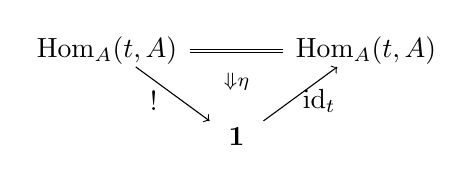
\begin{tikzpicture}[x=1.3em,y=1.3em]
  \node (L) at (0,0) {$\mathrm{Hom}_A(t,A)$};
  \node (R) at (7.2,0) {$\mathrm{Hom}_A(t,A)$};
  \node (one) at (3.6,-2.4) {$\qcOne$};
  \draw[double] (2.3,0) -- (4.9,0);
  \node at (3.6,-0.85) {$\scriptstyle\Downarrow\eta$};
  \draw[->] (0.8,-0.45) -- (2.85,-1.95);
  \node at (1.3,-1.4) {$!$};
  \draw[->] (4.35,-1.95) -- (6.4,-0.45);
  \node at (5.9,-1.4) {$\qcor{\mathrm{id}_t}$};
\end{tikzpicture}
\end{center}
以见证 $\qcor{\mathrm{id}_t}$ 的终性。由命题 3.4.6，我们可以用%
\trTwoCellInduction{}从一对满足相容性条件的\trNaturalTransformation{}
$(p_1\tau,\,p_0\tau)$ 归纳出 $\eta$。
这里必有 $p_0\tau=\mathrm{id}_{\qcOne}$，因为其余定义域∞-\trCategory{}是终的；
而我们定义 $p_1\tau$ 为 $\xi p_1$，其中 $\xi$ 是\trAdjunction{} $!\dashv t$
的\trUnit{}。命题 3.4.6(ii) 的相容性条件可由三角等式关系 $\xi_t=\mathrm{id}_t$
推出。
\end{proof}

分量 $\eta_{\qcor{\mathrm{id}_t}}$ 由一对恒等 2-\trCell{} $(\xi_t,\mathrm{id}_{\qcOne})$
诱导，故由\trTwoCellConservativity{}，$\eta_{\qcor{\mathrm{id}_t}}$ 可逆。由引理
2.2.2，这足以见证 $\qcor{\mathrm{id}_t}$ 的终性。

\trPointed{}\trInfinityCategory{}容许来自\trHomotopy{}论的若干熟知的构造。由%
定义 4.3.7，把点族 $\qcor{\rho}\colon A\to A^{2}$ 的两份副本沿其余定义域粘合，
便定义了一个余跨度族
$\mathring{\rho}\coloneqq\qcor{\rho}\vee\qcor{\rho}\colon A\to\Alc$。对偶地，
存在一个跨度族
$\mathring{\xi}\coloneqq\qcor{\xi}\wedge\qcor{\xi}\colon A\to\Arc$，它由把余点族
$\qcor{\xi}\colon A\to A^{2}$ 与其自身沿定义域粘合而定义。

\begin{definition}[\trLoops{}与\trSuspension]\label{def:loops-and-suspension}
一个\trPointed{}\trInfinityCategory{} $A$ 容许\textbf{\trLoops}（loops），
如果它容许余跨度族 $\mathring{\rho}$ 的一个\trLimit{}；此时\trLimit\trFunctor{}
$\Omega\colon A\to A$ 称为\textbf{\trLoops{}函子}（loops functor）。对偶地，一个%
\trPointed{}\trInfinityCategory{} $A$ 容许\textbf{\trSuspension}（suspensions），
如果它容许跨度族 $\mathring{\xi}$ 的一个\trColimit{}；此时%
\trColimit\trFunctor{} $\Sigma\colon A\to A$ 称为\textbf{\trSuspension{}函子}
（suspension functor）。
\end{definition}

\begin{center}
\begin{tikzpicture}[x=1.3em,y=1.3em]
  \node (A0) at (0,0) {$A$};
  \node (A1) at (4.4,2.3) {$A$};
  \node (AL) at (4.4,0) {$\Alc$};
  \draw[->,dashed] (0.45,0.3) -- (3.85,2.05);
  \node at (1.75,1.5) {$\Omega$};
  \node at (2.75,0.95) {$\scriptstyle\Downarrow$};
  \draw[->] (4.4,1.8) -- (4.4,0.5);
  \node at (4.95,1.15) {$\Delta$};
  \draw[->] (0.55,0) -- (3.8,0);
  \node at (2.15,-0.42) {$\mathring{\rho}$};
  \node at (7.3,1.15) {与};
  \begin{scope}[shift={(9.6,0)}]
  \node (B0) at (0,0) {$A$};
  \node (B1) at (4.4,2.3) {$A$};
  \node (AR) at (4.4,0) {$\Arc$};
  \draw[->,dashed] (0.45,0.3) -- (3.85,2.05);
  \node at (1.75,1.5) {$\Sigma$};
  \node at (2.75,0.95) {$\scriptstyle\Uparrow$};
  \draw[->] (4.4,1.8) -- (4.4,0.5);
  \node at (4.95,1.15) {$\Delta$};
  \draw[->] (0.55,0) -- (3.8,0);
  \node at (2.15,-0.42) {$\mathring{\xi}$};
  \end{scope}
\end{tikzpicture}
\end{center}

重要的是，若 $A$ 容许\trLoops{}与\trSuspension{}，则\trLoops{}函子与\trSuspension{}函子相互伴随：

\begin{proposition}[\trLoops--\trSuspension{}伴随]\label{prop:loops-suspension-adjunction}
若 $A$ 是一个容许\trLoops{}与\trSuspension{}的\trPointed{}\trInfinityCategory{}，则\trLoops{}函子是%
\trSuspension{}函子的\trRightAdjoint
\begin{center}
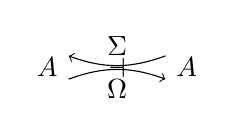
\begin{tikzpicture}[x=1.4em,y=1.4em]
  \node (L) at (0,0) {$A$};
  \node (R) at (3.6,0) {$A$};
  \draw[->] (3.05,0.3) to[bend left=20] node[above]{$\Sigma$} (0.55,0.3);
  \node at (1.8,0) {$\dashv$};
  \draw[->] (0.55,-0.3) to[bend left=20] node[below]{$\Omega$} (3.05,-0.3);
\end{tikzpicture}
\end{center}
\end{proposition}

证明的主要思想容易描述。如果 $A$ 容许一切\trPullback{}与一切\trPushout{}，那么%
推论 4.3.5 供应了诸\trAdjunction
\begin{center}
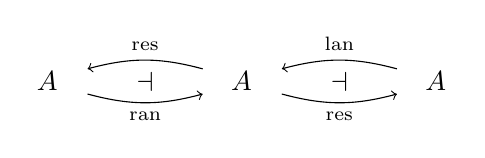
\begin{tikzpicture}[x=1.3em,y=1.3em]
  \node (L) at (0,0) {$\Alc$};
  \node (M) at (5.4,0) {$\Asq$};
  \node (R) at (10.8,0) {$\Arc$};
  \draw[->] (4.3,0.35) to[bend right=15] node[above]{$\scriptstyle\mathrm{res}$} (1.1,0.35);
  \node at (2.7,0) {$\dashv$};
  \draw[->] (1.1,-0.35) to[bend right=15] node[below]{$\scriptstyle\mathrm{ran}$} (4.3,-0.35);
  \draw[->] (9.7,0.35) to[bend right=15] node[above]{$\scriptstyle\mathrm{lan}$} (6.5,0.35);
  \node at (8.1,0) {$\dashv$};
  \draw[->] (6.5,-0.35) to[bend right=15] node[below]{$\scriptstyle\mathrm{res}$} (9.7,-0.35);
\end{tikzpicture}
\end{center}
它们在沿交换方块的中间顶点求值时纤维化于 $A\times A$ 之上。
沿 $(*,*)\colon\qcOne\to A\times A$ 作\trPullback{}，便把这些顶点钉于零元素处。
由于零元素既始又终，这种形式的拉回图表∞-\trCategory{}与推出图表%
∞-\trCategory{}都\trEquivalence{}于 $A$，而被拉回的诸伴随此刻便与\trLoops{}函子及%
\trSuspension{}函子重合。

随之而来的证明中唯一的微妙之处在于：我们作了更弱的假设——$A$ 只容许\trLoops{}与%
\trSuspension{}，而未必容许一切\trPullback{}与\trPushout{}。

\begin{proof}
余跨度族 $\mathring{\rho}$ 落入下方左图所定义的 $\Alc$ 的一个子对象
${\Alc}_{*}$ 之中，它由那些源元素被钉于 $A$ 的零元素 $*$ 处的余跨度组成。
\begin{center}
\begin{tikzpicture}[x=1.15em,y=1.15em]
  \node (A) at (0,2.6) {$A$};
  \node (AL) at (7.0,2.6) {$\Alc$};
  \node (ALs) at (3.5,0.7) {${\Alc}_{*}$};
  \node (one) at (0,-1.6) {$\qcOne$};
  \node (AA) at (7.0,-1.6) {$A\times A$};
  \draw[->] (1.0,2.85) to[bend left=12] node[above]{$\scriptstyle\mathring{\rho}$} (6.3,2.85);
  \draw[->,dashed] (0.55,2.2) -- (2.9,1.0);
  \node at (1.2,1.7) {$\scriptstyle\mathring{\rho}_{*}$};
  \draw[->] (4.3,0.85) -- (6.5,2.35);
  \draw[->] (3.1,0.5) -- (0.75,-1.2);
  \draw[->] (0,-2.1) -- (0,0.3);
  \draw[->] (7.0,-2.1) -- (7.0,1.3);
  \draw[->] (0.55,-1.6) -- (6.4,-1.6);
  \node at (3.5,-2.0) {$\scriptstyle(*,*)$};
  \node at (9.6,0.5) {与};
  \begin{scope}[shift={(11.4,0)}]
  \node (A2) at (0,2.6) {$A$};
  \node (H1) at (7.6,2.6) {$\mathrm{Hom}_A(*,A)$};
  \node (H2) at (0,-1.6) {$\mathrm{Hom}_A(*,A)$};
  \node (A3) at (7.6,-1.6) {$A$};
  \node (ALs2) at (3.8,0.7) {${\Alc}_{*}$};
  \draw[->] (1.0,2.85) to[bend left=12] node[above]{$\scriptstyle\qcor{\rho}$} (6.9,2.85);
  \node at (4.0,3.35) {$\scriptstyle\sim$};
  \draw[->,dashed] (0.55,2.2) -- (3.2,1.0);
  \node at (1.25,1.7) {$\scriptstyle\mathring{\rho}_{*}$};
  \draw[->] (4.6,0.85) -- (7.1,2.35);
  \node at (6.15,1.5) {$\scriptstyle\sim$};
  \draw[->] (3.45,0.55) -- (0.65,-1.25);
  \node at (1.7,-0.5) {$\scriptstyle *$};
  \draw[->,dashed] (0,-2.1) -- (0,2.1);
  \node at (-0.65,0.4) {$\scriptstyle\qcor{\rho}$};
  \draw[->] (7.6,2.1) -- (7.6,-2.1);
  \node at (8.25,0.4) {$\scriptstyle p_{1}$};
  \node at (8.0,1.15) {$\scriptstyle\sim$};
  \draw[->] (0.55,-1.6) -- (7.0,-1.6);
  \node at (3.8,-2.0) {$\scriptstyle p_{1}$};
  \node at (3.8,-1.2) {$\scriptstyle\sim$};
  \end{scope}
\end{tikzpicture}
\end{center}
由 ${\Alc}_{*}$ 的第二构造（如上方右图所示）连同命题 4.3.13 所给的始性刻画，
我们从\trEquivalence{}的\trTwoOfThreeProperty
首先得出：点族 $\qcor{\rho}\colon A\to A^{2}$ 经限制可定义一个\trEquivalence{}
$\qcor{\rho}\colon A\simeq\mathrm{Hom}_A(*,A)$，继而得出：诱导的图表
$\mathring{\rho}_{*}\colon A\simeq{\Alc}_{*}$ 是一个\trEquivalence{}。对偶地，
跨度族 $\mathring{\xi}\colon A\to\Arc$ 当把其余定义域限制到「靶元素被钉于零
元素 $*$ 处」的跨度子对象上时，定义一个\trEquivalence{}
$\mathring{\xi}_{*}\colon A\simeq{\Arc}_{*}$。

由命题 4.3.4，一个\trPointed{}\trInfinityCategory{} $A$ 容许\trLoops{}或容许\trSuspension{}，
当且仅当分别存在如下左图与如下右图所示的绝对\trLifting{}图
\begin{center}
\begin{tikzpicture}[x=1.2em,y=1.2em]
  \node (A0) at (0,0) {$A$};
  \node (Asq1) at (4.2,2.3) {$\Asq$};
  \node (AL1) at (4.2,0) {$\Alc$};
  \draw[->,dashed] (0.45,0.3) -- (3.75,2.05);
  \node at (1.5,1.5) {$\mathrm{ran}$};
  \node at (2.8,0.95) {$\scriptstyle\cong\Downarrow$};
  \draw[->] (4.2,1.8) -- (4.2,0.5);
  \node at (4.75,1.15) {$\mathrm{res}$};
  \draw[->] (0.55,0) -- (3.6,0);
  \node at (2.05,-0.42) {$\mathring{\rho}$};
  \node at (6.4,1.15) {与};
  \begin{scope}[shift={(8.6,0)}]
  \node (B0) at (0,0) {$A$};
  \node (Asq2) at (4.2,2.3) {$\Asq$};
  \node (AR1) at (4.2,0) {$\Arc$};
  \draw[->,dashed] (0.45,0.3) -- (3.75,2.05);
  \node at (1.5,1.5) {$\mathrm{lan}$};
  \node at (2.8,0.95) {$\scriptstyle\cong\Uparrow$};
  \draw[->] (4.2,1.8) -- (4.2,0.5);
  \node at (4.75,1.15) {$\mathrm{res}$};
  \draw[->] (0.55,0) -- (3.6,0);
  \node at (2.05,-0.42) {$\mathring{\xi}$};
  \end{scope}
\end{tikzpicture}
\end{center}
而且我们可以取这些自然同构为恒等。这样做使我们得以定义受限提升
\begin{center}
\begin{tikzpicture}[x=1.1em,y=1.1em]
  \node (AsqL) at (3.2,2.5) {$\Asq$};
  \node (AsqT) at (7.4,2.5) {$\Asq$};
  \node (A0) at (0,0) {$A$};
  \node (ALs) at (3.2,0) {${\Alc}_{*}$};
  \node (AL) at (7.4,0) {$\Alc$};
  \draw[->,dashed] (0.45,0.3) -- (2.8,2.2);
  \node at (1.0,1.5) {$\mathrm{ran}_{*}$};
  \node at (2.15,1.1) {$\scriptstyle\Vert$};
  \draw[->] (3.2,2.0) -- (3.2,0.55);
  \node at (3.85,1.25) {$\mathrm{res}_{*}$};
  \draw[->] (3.8,2.5) -- (6.8,2.5);
  \node at (5.3,2.5) {$\scriptstyle\hookrightarrow$};
  \draw[->] (7.4,2.0) -- (7.4,0.55);
  \node at (8.05,1.25) {$\mathrm{res}$};
  \draw[->] (0.55,0) -- (2.6,0);
  \node at (1.55,-0.42) {$\mathring{\rho}_{*}$};
  \draw[->] (3.8,0) -- (6.8,0);
  \node at (5.3,0) {$\scriptstyle\hookrightarrow$};
  \node at (9.6,1.25) {与};
  \begin{scope}[shift={(10.8,0)}]
  \node (AsqL) at (3.2,2.5) {$\Asq$};
  \node (AsqT) at (7.4,2.5) {$\Asq$};
  \node (A0) at (0,0) {$A$};
  \node (ARs) at (3.2,0) {${\Arc}_{*}$};
  \node (AR) at (7.4,0) {$\Arc$};
  \draw[->,dashed] (0.45,0.3) -- (2.8,2.2);
  \node at (1.0,1.5) {$\mathrm{lan}_{*}$};
  \node at (2.15,1.1) {$\scriptstyle\Vert$};
  \draw[->] (3.2,2.0) -- (3.2,0.55);
  \node at (3.85,1.25) {$\mathrm{res}_{*}$};
  \draw[->] (3.8,2.5) -- (6.8,2.5);
  \node at (5.3,2.5) {$\scriptstyle\hookrightarrow$};
  \draw[->] (7.4,2.0) -- (7.4,0.55);
  \node at (8.05,1.25) {$\mathrm{res}$};
  \draw[->] (0.55,0) -- (2.6,0);
  \node at (1.55,-0.42) {$\mathring{\xi}_{*}$};
  \draw[->] (3.8,0) -- (6.8,0);
  \node at (5.3,0) {$\scriptstyle\hookrightarrow$};
  \end{scope}
\end{tikzpicture}
\end{center}
并且我们再次论证它们分别定义绝对右与绝对左\trLifting{}图。右手与左手的论证
互为对偶，故我们把注意力集中于前者。由定理 3.5.3，这张绝对右\trLifting{}图
定义
一个纤维化\trEquivalence{}
$\mathrm{Hom}_{\Asq}(\Asq,\mathrm{ran})\simeq_{A\times\Asq}\mathrm{Hom}_{\Alc}(\mathrm{res},\mathring{\rho})$，
它可以沿「中间顶点被钉于零元素处的、$A$ 中的交换方块」之子对象
${\Asq}_{*}\hookrightarrow\Asq$ 的含入作\trPullback{}，从而给出一个纤维化于
$A\times{\Asq}_{*}$ 之上的\trEquivalence{}。我们断言：这些∞-\trCategory{}经%
\trPullback{}所得的∞-\trCategory{}分别\trEquivalence{}于
$\mathrm{Hom}_{{\Asq}_{*}}({\Asq}_{*},\mathrm{ran}_{*})$ 与
$\mathrm{Hom}_{{\Alc}_{*}}(\mathrm{res}_{*},\mathring{\rho}_{*})$。

为看出这一点，首先注意到零元素的\trUniversalProperty{}蕴含
$\mathrm{Hom}_A(*,*)$ 可缩（见命题 4.3.13），
因而外方块\trEquivalence{}于如下\trPullback
\begin{center}
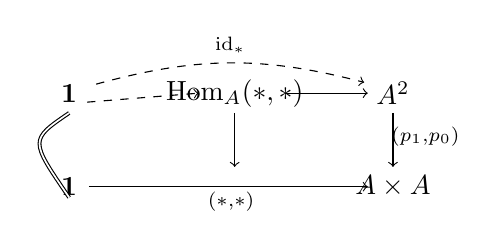
\begin{tikzpicture}[x=1.3em,y=1.3em]
  \node (one1) at (0,2.3) {$\qcOne$};
  \node (Hom) at (4.6,2.3) {$\mathrm{Hom}_A(*,*)$};
  \node (A2) at (9.0,2.3) {$A^{2}$};
  \node (one2) at (0,-0.3) {$\qcOne$};
  \node (AA) at (9.0,-0.3) {$A\times A$};
  \draw[->,dashed] (0.75,2.55) to[bend left=15] node[above]{$\scriptstyle\qcor{\mathrm{id}_*}$} (8.2,2.6);
  \draw[->,dashed] (0.5,2.05) -- (3.6,2.3);
  \draw[->] (6.0,2.3) -- (8.3,2.3);
  \node at (3.3,1.35) {$\scriptstyle\lrcorner$};
  \draw[double] (0,-0.6) .. controls (-1.1,1.0) .. (0,1.75);
  \draw[->] (4.6,1.75) -- (4.6,0.25);
  \draw[->] (9.0,1.75) -- (9.0,0.25);
  \node at (9.9,1.1) {$\scriptstyle(p_{1},p_{0})$};
  \draw[->] (0.55,-0.3) -- (8.3,-0.3);
  \node at (4.5,-0.72) {$\scriptstyle(*,*)$};
\end{tikzpicture}
\end{center}
由于这一交换棱柱的顶面与底面都是严格\trPullback
\begin{center}
\begin{tikzpicture}[x=1.0em,y=1.0em]
  \node (t1) at (0,4.6) {$(\Asq)^{2}$};
  \node (t2) at (6.4,4.6) {$(\Alc)^{2}$};
  \node (t3) at (14.4,4.6) {$A^{2}\times A^{2}$};
  \node (m1) at (-3.4,2.3) {$({\Asq}_{*})^{2}$};
  \node (m2) at (3.0,2.3) {$({\Alc}_{*})^{2}$};
  \node (m3) at (10.4,2.3) {$\qcOne$};
  \node (b1) at (-3.4,0) {$\Asq\times\Asq$};
  \node (b2) at (3.0,0) {$\Alc\times\Alc$};
  \node (b3) at (14.4,0) {$A\times A\times A\times A$};
  \node (b4) at (-3.4,-2.3) {${\Asq}_{*}\times{\Asq}_{*}$};
  \node (b5) at (3.0,-2.3) {${\Alc}_{*}\times{\Alc}_{*}$};
  \node (b6) at (10.4,-2.3) {$\qcOne$};
  \draw[->] (1.6,4.6) -- node[above]{$\scriptstyle\mathrm{res}^{2}$} (4.6,4.6);
  \draw[->] (8.2,4.6) -- (12.6,4.6);
  \draw[->] (-2.4,2.3) -- node[above]{$\scriptstyle\mathrm{res}_{*}^{2}$} (1.4,2.3);
  \node at (-0.5,2.75) {$\scriptstyle\lrcorner$};
  \draw[->] (4.7,2.3) -- (8.6,2.3);
  \node at (6.6,2.75) {$\scriptstyle\lrcorner$};
  \draw[->] (-3.4,1.75) -- (-3.4,0.55);
  \draw[->] (3.0,1.75) -- (3.0,0.55);
  \draw[->] (10.95,2.6) -- node[above]{$\scriptstyle(\mathrm{id}_{*},\mathrm{id}_{*})$} node[below,pos=0.3]{$\scriptstyle\sim$} (13.4,4.25);
  \draw[->] (-1.0,0) -- node[above]{$\scriptstyle\mathrm{res}\times\mathrm{res}$} (1.4,0);
  \draw[->] (4.9,0) -- (11.9,0.35);
  \draw[right hook->] (-3.4,-1.75) -- (-3.4,-0.55);
  \draw[->] (-1.2,-2.3) -- node[above]{$\scriptstyle\mathrm{res}_{*}\times\mathrm{res}_{*}$} (1.2,-2.3);
  \draw[->] (5.0,-2.3) -- (9.8,-2.3);
  \draw[->] (10.9,-2.05) -- node[below]{$\scriptstyle(*,*,*)$} (13.5,-0.45);
  \draw[->] (-2.6,2.0) -- (-1.2,4.3);
  \draw[->] (3.8,2.0) -- (5.2,4.3);
  \draw[->] (-2.6,-0.3) -- (-1.4,-1.9);
  \draw[right hook->] (5.0,-1.9) -- (3.8,-0.3);
\end{tikzpicture}
\end{center}
由此推出：其左侧面与中侧面也在\trEquivalence{}意义下成为\trPullback{}。我们
使用其中的后一侧面以及如下交换立方
\begin{center}
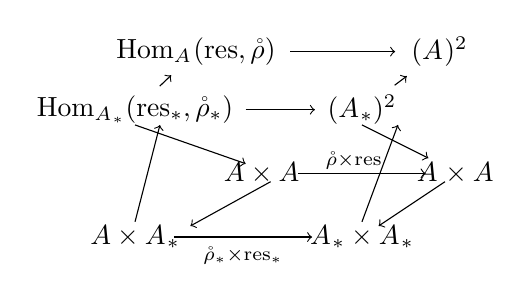
\begin{tikzpicture}[x=1.0em,y=1.0em]
  \node (cTL) at (2.2,4.4) {$\mathrm{Hom}_{\Alc}(\mathrm{res},\mathring{\rho})$};
  \node (cTR) at (11.0,4.4) {$(\Alc)^{2}$};
  \node (cBL) at (0,2.3) {$\mathrm{Hom}_{{\Alc}_{*}}(\mathrm{res}_{*},\mathring{\rho}_{*})$};
  \node (cBR) at (8.2,2.3) {$({\Alc}_{*})^{2}$};
  \node (dM) at (4.6,0) {$A\times\Asq$};
  \node (dR) at (11.6,0) {$\Alc\times\Alc$};
  \node (eL) at (0,-2.3) {$A\times{\Asq}_{*}$};
  \node (eR) at (8.2,-2.3) {${\Alc}_{*}\times{\Alc}_{*}$};
  \draw[->] (5.6,4.4) -- (9.4,4.4);
  \node at (5.1,3.5) {$\scriptstyle\lrcorner$};
  \draw[->] (4.0,2.3) -- (6.5,2.3);
  \node at (1.2,3.4) {$\scriptstyle\lrcorner$};
  \draw[->] (cBL) -- (cTL);
  \draw[->] (cBR) -- (cTR);
  \draw[->] (0,1.75) -- (4.0,0.35);
  \draw[->] (8.2,1.75) -- (10.6,0.55);
  \node at (7.9,0.45) {$\scriptstyle\mathring{\rho}\times\mathrm{res}$};
  \draw[->] (5.9,0) -- (10.5,0);
  \draw[->] (1.4,-2.3) -- node[below]{$\scriptstyle\mathring{\rho}_{*}\times\mathrm{res}_{*}$} (6.4,-2.3);
  \node at (3.2,-1.35) {$\scriptstyle\lrcorner$};
  \draw[->] (0,-1.75) -- (0.9,1.75);
  \draw[->] (8.2,-1.75) -- (9.5,1.75);
  \draw[->] (4.9,-0.3) -- (2.0,-1.9);
  \draw[->] (11.2,-0.3) -- (8.8,-1.9);
\end{tikzpicture}
\end{center}
以断定：由含入 ${\Asq}_{*}\hookrightarrow\Asq$ 取\trPullback{}所得的
逗号∞-\trCategory{} $\mathrm{Hom}_{\Alc}(\mathrm{res},\mathring{\rho})$
\trEquivalence{}于 $\mathrm{Hom}_{{\Alc}_{*}}(\mathrm{res}_{*},\mathring{\rho}_{*})$，
一如所断言。
类似地，由前一个在\trEquivalence{}意义下的\trPullback{}，我们断定
$\mathrm{Hom}_{\Asq}(\Asq,\mathrm{ran})$ 的\trPullback\trEquivalence{}于
$\mathrm{Hom}_{{\Asq}_{*}}({\Asq}_{*},\mathrm{ran}_{*})$。

这样我们便得到纤维化\trEquivalence
\begin{center}
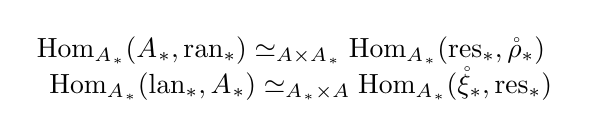
\begin{tikzpicture}[x=1.0em,y=1.0em]
  \node at (0,1.2) {$\mathrm{Hom}_{{\Asq}_{*}}({\Asq}_{*},\mathrm{ran}_{*})\simeq_{A\times{\Asq}_{*}}\mathrm{Hom}_{{\Alc}_{*}}(\mathrm{res}_{*},\mathring{\rho}_{*})$};
  \node at (0.35,0) {$\mathrm{Hom}_{{\Asq}_{*}}(\mathrm{lan}_{*},{\Asq}_{*})\simeq_{{\Asq}_{*}\times A}\mathrm{Hom}_{{\Arc}_{*}}(\mathring{\xi}_{*},\mathrm{res}_{*})$};
\end{tikzpicture}
\end{center}
据定理 3.5.8，它们经由诸限制\trFunctor{}编码了 $\mathring{\rho}_{*}$ 与
$\mathring{\xi}_{*}$ 的绝对提升：
\begin{center}
\begin{tikzpicture}[x=1.05em,y=1.05em]
  \node (a0) at (0,0) {$A$};
  \node (a1) at (3.6,2.2) {$\Asq$};
  \node (a2) at (3.6,0) {$\Alc$};
  \draw[->,dashed] (0.4,0.3) -- (3.15,1.95);
  \node at (1.2,1.4) {$\mathrm{ran}_{*}$};
  \node at (2.3,0.95) {$\scriptstyle\cong\Downarrow$};
  \draw[->] (3.6,1.7) -- (3.6,0.5);
  \node at (4.2,1.1) {$\mathrm{res}_{*}$};
  \draw[->] (0.55,0) -- (3.0,0);
  \node at (1.8,-0.42) {$\mathring{\rho}_{*}$};
  \node at (5.3,1.1) {$\;\rightsquigarrow$};
  \begin{scope}[shift={(6.6,0)}]
  \node (b0) at (0,0) {$\Alc$};
  \node (b1) at (3.6,2.2) {$\Asq$};
  \node (b2) at (3.6,0) {$\Alc$};
  \draw[->,dashed] (0.4,0.3) -- (3.15,1.95);
  \node at (1.2,1.4) {$\mathrm{ran}_{*}$};
  \node at (2.3,0.95) {$\scriptstyle\cong\Downarrow$};
  \draw[->] (3.6,1.7) -- (3.6,0.5);
  \node at (4.2,1.1) {$\mathrm{res}_{*}$};
  \draw[double] (0.6,0) -- (3.0,0);
  \end{scope}
  \node at (12.2,1.1) {与};
  \begin{scope}[shift={(13.6,0)}]
  \node (c0) at (0,0) {$A$};
  \node (c1) at (3.6,2.2) {$\Asq$};
  \node (c2) at (3.6,0) {$\Arc$};
  \draw[->,dashed] (0.4,0.3) -- (3.15,1.95);
  \node at (1.2,1.4) {$\mathrm{lan}_{*}$};
  \node at (2.3,0.95) {$\scriptstyle\cong\Uparrow$};
  \draw[->] (3.6,1.7) -- (3.6,0.5);
  \node at (4.2,1.1) {$\mathrm{res}_{*}$};
  \draw[->] (0.55,0) -- (3.0,0);
  \node at (1.8,-0.42) {$\mathring{\xi}_{*}$};
  \node at (5.3,1.1) {$\;\rightsquigarrow$};
  \begin{scope}[shift={(6.6,0)}]
  \node (d0) at (0,0) {$\Arc$};
  \node (d1) at (3.6,2.2) {$\Asq$};
  \node (d2) at (3.6,0) {$\Arc$};
  \draw[->,dashed] (0.4,0.3) -- (3.15,1.95);
  \node at (1.2,1.4) {$\mathrm{lan}_{*}$};
  \node at (2.3,0.95) {$\scriptstyle\cong\Uparrow$};
  \draw[->] (3.6,1.7) -- (3.6,0.5);
  \node at (4.2,1.1) {$\mathrm{res}_{*}$};
  \draw[double] (0.6,0) -- (3.0,0);
  \end{scope}
  \end{scope}
\end{tikzpicture}
\end{center}
沿\trEquivalence{} ${\Alc}_{*}\simeq A$ 与 ${\Arc}_{*}\simeq A$ 之逆限制到
$\mathring{\rho}_{*}$ 与 $\mathring{\xi}_{*}$ 上，并与可逆 2-\trCell{}粘贴，
我们便得到底边为恒等的绝对\trLifting{}图。

由引理 2.3.7，这些\trLifting{}图定义了诸\trAdjunction{}：
\begin{center}
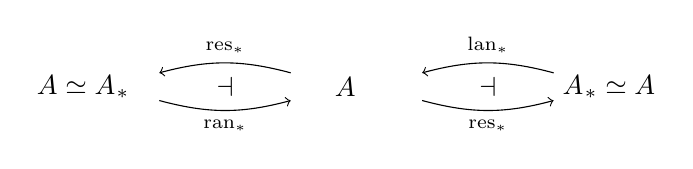
\begin{tikzpicture}[x=1.25em,y=1.25em]
  \node (p) at (0,0) {$A\simeq{\Alc}_{*}$};
  \node (q) at (7.6,0) {$\Asq$};
  \node (r) at (15.2,0) {${\Arc}_{*}\simeq A$};
  \draw[->] (6.0,0.4) to[bend right=15] node[above]{$\scriptstyle\mathrm{res}_{*}$} (2.2,0.4);
  \node at (4.1,0) {$\dashv$};
  \draw[->] (2.2,-0.4) to[bend right=15] node[below]{$\scriptstyle\mathrm{ran}_{*}$} (6.0,-0.4);
  \draw[->] (13.6,0.4) to[bend right=15] node[above]{$\scriptstyle\mathrm{lan}_{*}$} (9.8,0.4);
  \node at (11.7,0) {$\dashv$};
  \draw[->] (9.8,-0.4) to[bend right=15] node[below]{$\scriptstyle\mathrm{res}_{*}$} (13.6,-0.4);
\end{tikzpicture}
\end{center}
它们复合出所要的\trAdjunction{} $\Sigma\dashv\Omega$。
\end{proof}

\begin{definition}[纤维与余纤维]\label{def:fiber-and-cofiber}
\trPointed{}\trInfinityCategory{} $A$ 中的一个从 $x$ 到 $y$ 的箭头
$f\colon\qcOne\to A^{2}$ \textbf{容许纤维}（admits a fiber），如果 $A$ 容许
由 $f$ 与点族的分量 $\qcor{\rho_y}$ 所成余跨度的一个\trPullback{}。由绝对右%
\trLifting{}图
\begin{center}
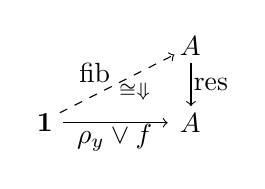
\begin{tikzpicture}[x=1.2em,y=1.2em]
  \node (one) at (0,0) {$\qcOne$};
  \node (Asq) at (4.4,2.3) {$\Asq$};
  \node (AL) at (4.4,0) {$\Alc$};
  \draw[->,dashed] (0.45,0.3) -- (3.9,2.05);
  \node at (1.5,1.5) {$\mathrm{fib}$};
  \node at (2.7,0.95) {$\scriptstyle\cong\Downarrow$};
  \draw[->] (4.4,1.8) -- (4.4,0.5);
  \node at (5.0,1.15) {$\mathrm{res}$};
  \draw[->] (0.55,0) -- (3.7,0);
  \node at (2.1,-0.45) {$\qcor{\rho_{y}}\vee f$};
\end{tikzpicture}
\end{center}
所定义的\trPullback{}方块称为 $f$ 的\textbf{纤维序列}（fiber sequence）。
对偶地，$f$ \textbf{容许余纤维}（admits a cofiber），如果 $A$ 容许由 $f$ 与
余点族的分量 $\qcor{\xi_x}$ 所成跨度的一个\trPushout{}；此时\trPushout{}方块
\begin{center}
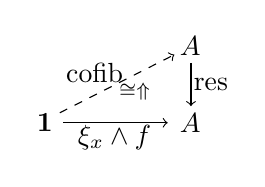
\begin{tikzpicture}[x=1.2em,y=1.2em]
  \node (one) at (0,0) {$\qcOne$};
  \node (Asq) at (4.4,2.3) {$\Asq$};
  \node (AR) at (4.4,0) {$\Arc$};
  \draw[->,dashed] (0.45,0.3) -- (3.9,2.05);
  \node at (1.5,1.5) {$\mathrm{cofib}$};
  \node at (2.7,0.95) {$\scriptstyle\cong\Uparrow$};
  \draw[->] (4.4,1.8) -- (4.4,0.5);
  \node at (5.0,1.15) {$\mathrm{res}$};
  \draw[->] (0.55,0) -- (3.7,0);
  \node at (2.1,-0.45) {$\qcor{\xi_{x}}\wedge f$};
\end{tikzpicture}
\end{center}
定义 $f$ 的\textbf{余纤维序列}（cofiber sequence）。
\end{definition}

$A$ 中的纤维序列与余纤维序列定义了左下顶点为零元素 $*$ 的交换方块：
\begin{center}
\begin{tikzpicture}[x=1.3em,y=1.3em]
  \node (fb) at (0,2.2) {$\mathrm{fib}(f)$};
  \node (x) at (4.4,2.2) {$x$};
  \node (st) at (0,0) {$*$};
  \node (y) at (4.4,0) {$y$};
  \draw[->] (1.1,2.2) -- (3.7,2.2);
  \draw[->] (0,1.65) -- (0,0.55);
  \draw[->] (4.4,1.65) -- (4.4,0.55);
  \node at (4.95,1.1) {$f$};
  \draw[->] (0.55,0) -- (3.7,0);
  \node at (2.15,1.3) {$\scriptstyle\lrcorner$};
  \node at (7.1,1.1) {与};
  \begin{scope}[shift={(9.4,0)}]
  \node (x2) at (0,2.2) {$x$};
  \node (y2) at (4.4,2.2) {$y$};
  \node (st2) at (0,0) {$*$};
  \node (cf) at (5.6,0) {$\mathrm{cofib}(f)$};
  \draw[->] (0.6,2.2) -- node[above]{$f$} (3.7,2.2);
  \draw[->] (0,1.65) -- (0,0.55);
  \draw[->] (4.4,1.9) -- (5.2,0.55);
  \draw[->] (0.55,0) -- (4.5,0);
  \node at (2.5,1.3) {$\scriptstyle\ulcorner$};
  \end{scope}
\end{tikzpicture}
\end{center}
这些方块的数据由 $A$ 中的一个交换三角形——即 $A^{3}$ 的一个\trElement{}——
给出，其中涉及一条我们未曾画出的对角箭头，连同该对角边的%
\textbf{\trNullhomotopy}（nullhomotopy）——即这条边经由零元素分解于 $\mathrm{h}A$ 中的
一个见证。左下顶点为零元素的 $A$ 中交换方块称为 $A$ 中的一个
\textbf{三角形}（triangle）。

现在我们可以陈述\trStable{}\trInfinityCategory{}的第一批彼此\trEquivalence{}%
的刻画中的第一个。这一概念及其后的结果归功于 Lurie，最初出现于预印本
\cite{bib77}中，后收编入 \emph{Higher Algebra} \cite{bib80}的第一章。

\begin{definition}[\trStable{}\trInfinityCategory]\label{def:stable-infinity-category}
一个\textbf{稳定的∞-范畴}（stable ∞-category）是一个\trPointed{}\trInfinityCategory{} $A$，使得
\begin{itemize}
\item[(i)] 每个态射都容许一个纤维与一个余纤维：也就是说，存在绝对\trLifting{}图
\begin{center}
\begin{tikzpicture}[x=1.15em,y=1.15em]
  \node (A2) at (0,0) {$A^{2}$};
  \node (Asq) at (4.2,2.3) {$\Asq$};
  \node (AL) at (4.2,0) {$\Alc$};
  \draw[->,dashed] (0.45,0.3) -- (3.7,2.05);
  \node at (1.4,1.5) {$\mathrm{fib}$};
  \node at (2.6,1.0) {$\scriptstyle\cong\Downarrow$};
  \draw[->] (4.2,1.8) -- (4.2,0.5);
  \node at (4.8,1.15) {$\mathrm{res}$};
  \draw[->] (0.6,0) -- (3.5,0);
  \node at (2.05,-0.45) {$\qcor{\rho_{\mathrm{cod}}}\vee\mathrm{id}$};
  \node at (6.9,1.15) {与};
  \begin{scope}[shift={(9.2,0)}]
  \node (B2) at (0,0) {$A^{2}$};
  \node (Bsq) at (4.2,2.3) {$\Asq$};
  \node (BR) at (4.2,0) {$\Arc$};
  \draw[->,dashed] (0.45,0.3) -- (3.7,2.05);
  \node at (1.4,1.5) {$\mathrm{cofib}$};
  \node at (2.6,1.0) {$\scriptstyle\cong\Uparrow$};
  \draw[->] (4.2,1.8) -- (4.2,0.5);
  \node at (4.8,1.15) {$\mathrm{res}$};
  \draw[->] (0.6,0) -- (3.5,0);
  \node at (2.05,-0.45) {$\qcor{\xi_{\mathrm{dom}}}\wedge\mathrm{id}$};
  \end{scope}
\end{tikzpicture}
\end{center}
\item[(ii)] 以及：$A$ 中的一个三角形定义一个纤维序列，当且仅当它也定义一个余纤维
序列。这样的三角形称为\textbf{正合三角形}（exact triangles）。
\end{itemize}
\end{definition}

作为熟悉这一定义的一种途径，我们证明：

\begin{lemma}\label{lem:diagram-stable}
设 $A$ 是一个\trStable{}\trInfinityCategory{}，并设 $J$ 为一个\trSimplicialSet{}，
或者在周围∞-\trInfinityCosmos{} $\mathcal{K}$ \trCartesianClosed{}时
取 $J$ 为另一个∞-\trCategory{}。则 $A^{J}$ 仍是\trStable{}\trInfinityCategory{}。
\end{lemma}

\begin{proof}
由命题 2.1.7，\trCosmologicalFunctor{} $(-)^{J}\colon\mathcal{K}\to\mathcal{K}$
保持诸\trAdjunction
\begin{center}
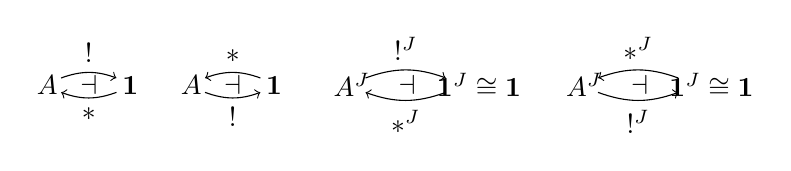
\begin{tikzpicture}[x=1.0em,y=1.0em]
  \node (A1) at (0,0) {$A$};
  \node (o1) at (3.0,0) {$\qcOne$};
  \draw[->] (0.5,0.26) to[bend left=20] node[above]{$!$} (2.5,0.26);
  \node at (1.5,0) {$\dashv$};
  \draw[->] (2.5,-0.26) to[bend left=20] node[below]{$*$} (0.5,-0.26);
  \begin{scope}[shift={(5.2,0)}]
  \node (A2) at (0,0) {$A$};
  \node (o2) at (3.0,0) {$\qcOne$};
  \draw[->] (2.5,0.26) to[bend right=20] node[above]{$*$} (0.5,0.26);
  \node at (1.5,0) {$\dashv$};
  \draw[->] (0.5,-0.26) to[bend right=20] node[below]{$!$} (2.5,-0.26);
  \end{scope}
  \node at (9.3,0) {$\rightsquigarrow$};
  \begin{scope}[shift={(11.0,0)}]
  \node (A3) at (0,0) {$A^{J}$};
  \node (o3) at (4.6,0) {$\qcOne^{J}\cong\qcOne$};
  \draw[->] (0.5,0.26) to[bend left=20] node[above]{$!^{J}$} (3.4,0.26);
  \node at (2.0,0) {$\dashv$};
  \draw[->] (3.4,-0.26) to[bend left=20] node[below]{$*^{J}$} (0.5,-0.26);
  \begin{scope}[shift={(8.4,0)}]
  \node (A4) at (0,0) {$A^{J}$};
  \node (o4) at (4.6,0) {$\qcOne^{J}\cong\qcOne$};
  \draw[->] (3.4,0.26) to[bend right=20] node[above]{$*^{J}$} (0.5,0.26);
  \node at (2.0,0) {$\dashv$};
  \draw[->] (0.5,-0.26) to[bend right=20] node[below]{$!^{J}$} (3.4,-0.26);
  \end{scope}
  \end{scope}
\end{tikzpicture}
\end{center}
它们展示零元素 $*\colon\qcOne\to A$ 的\trUniversalProperty{}。这样，我们看到
$A^{J}$ 是一个\trPointed{}\trInfinityCategory{}，其基点是取值于 $*$ 的常值
$J$ 形\trFunctor{}。

类似地，由推论 3.5.7，\trCosmologicalFunctor{}
$(-)^{J}\colon\mathcal{K}\to\mathcal{K}$ 保持定义纤维序列与余纤维序列的
\cref{def:stable-infinity-category}(i) 之绝对\trLifting{}图。
由于 $\mathrm{res}^{J}\colon(\Asq)^{J}\to(\Alc)^{J}$ 同构于
$\mathrm{res}\colon(A^{J})^{\square}\to(A^{J})^{\llcorner}$，且把方块限制到
其底跨度的\trFunctor{}亦然，这些绝对\trLifting{}图便定义 $A^{J}$ 中的纤维
序列与余纤维序列。

最后，\cref{def:stable-infinity-category}(ii) 的条件可以重新表述为：下方左图
所示的交换三角形是绝对左提升的，而下方右图所示的三角形是绝对右提升的：
\begin{center}
\begin{tikzpicture}[x=1.15em,y=1.15em]
  \node (A2) at (0,0) {$A^{2}$};
  \node (Asq) at (4.2,2.3) {$\Asq$};
  \node (AR) at (4.2,0) {$\Arc$};
  \draw[->,dashed] (0.45,0.3) -- (3.7,2.05);
  \node at (1.4,1.5) {$\mathrm{fib}$};
  \node at (2.5,1.05) {$\scriptstyle\Vert$};
  \draw[->] (4.2,1.8) -- (4.2,0.5);
  \node at (4.8,1.15) {$\mathrm{res}$};
  \draw[->] (0.6,0) -- (3.5,0);
  \node at (2.0,-0.45) {$\mathrm{res}\circ\mathrm{fib}$};
  \node at (6.9,1.15) {与};
  \begin{scope}[shift={(9.2,0)}]
  \node (B2) at (0,0) {$A^{2}$};
  \node (Bsq) at (4.2,2.3) {$\Asq$};
  \node (BL) at (4.2,0) {$\Alc$};
  \draw[->,dashed] (0.45,0.3) -- (3.7,2.05);
  \node at (1.4,1.5) {$\mathrm{cofib}$};
  \node at (2.5,1.05) {$\scriptstyle\Vert$};
  \draw[->] (4.2,1.8) -- (4.2,0.5);
  \node at (4.8,1.15) {$\mathrm{res}$};
  \draw[->] (0.6,0) -- (3.5,0);
  \node at (2.0,-0.45) {$\mathrm{res}\circ\mathrm{cofib}$};
  \end{scope}
\end{tikzpicture}
\end{center}
也就是说：$A$ 中的纤维序列也是余纤维序列，而 $A$ 中的余纤维序列也是纤维
序列。再一次应用推论 3.5.7，我们看到同样的正合性质在 $A^{J}$ 中成立。因此
$A^{J}$ 是稳定的。
\end{proof}

\trStable{}\trInfinityCategory{}事实上容许一切\trPushout{}与一切%
\trPullback{}，而且这样的方块相互重合。既是\trPushout{}又是\trPullback{}的
方块称为\textbf{\trExactSquare}（exact squares）。

\begin{proposition}[\trStable{}\trInfinityCategory{}中的\trPullback{}与%
\trPushout]\label{prop:pb-po-stable}
\trStable{}\trInfinityCategory{}容许一切\trPushout{}与一切\trPullback{}；而且，
一个方块是\trPushout{}，当且仅当它是一个\trPullback{}。
\end{proposition}

\begin{proof}
给定 $A$ 中余跨度的一般族 $g\vee f\colon X\to\Alc$，先作 $f$ 的余纤维，再作
复合映射 $qg\colon c\to a\to\mathrm{cofib}\,f$ 的纤维：
\begin{rveq}\label{eq:fib-qg-rectangle}
\mbox{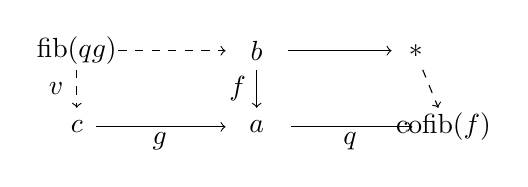
\begin{tikzpicture}[x=1.25em,y=1.25em]
  \node (fq) at (0,2.2) {$\mathrm{fib}(qg)$};
  \node (b) at (5.2,2.2) {$b$};
  \node (st) at (9.8,2.2) {$*$};
  \node (c) at (0,0) {$c$};
  \node (a) at (5.2,0) {$a$};
  \node (cf) at (10.6,0) {$\mathrm{cofib}(f)$};
  \draw[->,dashed] (1.2,2.2) -- (4.3,2.2);
  \draw[->] (6.1,2.2) -- (9.1,2.2);
  \draw[->,dashed] (0,1.65) -- (0,0.55);
  \node at (-0.6,1.1) {$v$};
  \draw[->] (5.2,1.65) -- (5.2,0.55);
  \node at (4.65,1.1) {$f$};
  \draw[->,dashed] (10.0,1.65) -- (10.45,0.55);
  \draw[->] (0.55,0) -- (4.3,0);
  \node at (2.4,-0.42) {$g$};
  \draw[->] (6.2,0) -- (9.7,0);
  \node at (7.9,-0.42) {$q$};
  \node at (2.4,1.3) {$\scriptstyle\lrcorner$};
  \node at (7.9,1.3) {$\scriptstyle\ulcorner$};
\end{tikzpicture}}
\end{rveq}
由\cref{def:stable-infinity-category}(ii)，余纤维序列
$b\to a\to\mathrm{cofib}(f)$ 也是一个纤维序列。
由命题 4.3.11 的拉回消去结果，我们断定 $\mathrm{fib}(qg)$ 计算出余跨度
$g\vee f$ 的\trPullback{}。
为看出这个\trPullback{}方块也是一个\trPushout{}，作映射 $v$ 的纤维：
\begin{center}
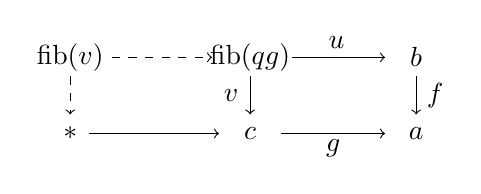
\begin{tikzpicture}[x=1.25em,y=1.25em]
  \node (fv) at (0,2.2) {$\mathrm{fib}(v)$};
  \node (fq) at (5.2,2.2) {$\mathrm{fib}(qg)$};
  \node (b) at (10.0,2.2) {$b$};
  \node (st) at (0,0) {$*$};
  \node (c) at (5.2,0) {$c$};
  \node (a) at (10.0,0) {$a$};
  \draw[->,dashed] (1.2,2.2) -- (4.1,2.2);
  \draw[->] (6.4,2.2) -- (9.1,2.2);
  \node at (7.7,2.62) {$u$};
  \draw[->,dashed] (0,1.65) -- (0,0.55);
  \draw[->] (5.2,1.65) -- (5.2,0.55);
  \node at (4.65,1.1) {$v$};
  \draw[->] (10.0,1.65) -- (10.0,0.55);
  \node at (10.55,1.1) {$f$};
  \draw[->] (0.55,0) -- (4.3,0);
  \draw[->] (6.1,0) -- (9.1,0);
  \node at (7.6,-0.42) {$g$};
  \node at (1.7,1.3) {$\scriptstyle\lrcorner$};
  \node at (6.9,1.3) {$\scriptstyle\lrcorner$};
\end{tikzpicture}
\end{center}
由命题 4.3.11 的拉回复合结果，$\mathrm{fib}(v)$ 也是映射 $f$ 的纤维。由%
\cref{def:stable-infinity-category}(ii)，纤维序列
$\mathrm{fib}(v)\to\mathrm{fib}(qg)\to c$ 与
$\mathrm{fib}(v)\to b\to a$ 也是余纤维序列。再由命题 4.3.11 的推出消去
结果，我们看到右手边的\trPullback{}方块也是一个\trPushout{}方块。一个对偶
论证证明\trPushout{}存在并与\trPullback{}重合。
\end{proof}

\begin{digression}[用广义元素定义\trFunctor]\label{dig:generalized-elements-functors}
刚才所给证明的第一段取余跨度的一般族并构造了一个矩形图表
\cref{eq:fib-qg-rectangle}，命题 4.3.11 可应用于其上（据注 4.3.12）。
由\trYonedaLemma{}，一个作为广义元素上的映射给出的构造在∞-\trInfinityCosmos{}%
内部定义一个箭头，在此情形下取\trFunctor{} $\Alc\to A^{3\times 2}$ 的形式，
我们现在通过拆解每一步来阐明这一点。\footnote{诚然，这个\trFunctor{}可以理解为把
该构造应用于泛广义元素的结果，此时一切都由恒同给出。以一般余跨度
$g\vee f\colon X\to\Alc$ 代替泛余跨度 $\mathrm{id}\colon\Alc\to\Alc$ 的用意，
在于引入一些人类可读的记号。}首先，我们从一般余跨度构造下方左图的虚线箭头，
它构成的图表把这个余跨度粘合到其一条腿所关联的余纤维序列上：
\begin{center}
\begin{tikzpicture}[x=1.05em,y=1.05em]
  \node (A2t) at (3.4,4.0) {$A^{2}$};
  \node (ALl) at (-1.8,1.7) {$\Alc$};
  \node (ALd) at (3.4,1.7) {$A^{\llcorner\square}$};
  \node (Asq) at (8.6,1.7) {$\Asq$};
  \node (ALb) at (3.4,-0.9) {$\Alc$};
  \node (A2b) at (8.6,-0.9) {$A^{2}$};
  \draw[->] (-0.8,2.15) -- node[above left]{$\scriptstyle\mathrm{res}_{\llcorner}$} (2.8,3.75);
  \draw[->] (4.1,3.75) -- node[above right]{$\scriptstyle\mathrm{cofib}$} (7.9,2.15);
  \draw[->,dashed] (-0.7,1.7) -- (2.3,1.7);
  \draw[->] (4.5,1.7) -- (7.5,1.7);
  \draw[double] (-1.4,1.45) -- (2.7,-0.65);
  \draw[->] (3.4,1.15) -- (3.4,-0.35);
  \node at (4.05,0.4) {$\scriptstyle\lrcorner$};
  \draw[->] (8.6,1.15) -- node[right]{$\scriptstyle\mathrm{res}_{\llcorner}$} (8.6,-0.35);
  \draw[->] (4.0,-0.9) -- node[below]{$\scriptstyle\mathrm{res}_{\llcorner}$} (7.9,-0.9);
  \node at (12.0,1.4) {与};
  \begin{scope}[shift={(13.4,0)}]
  \node (B2t) at (4.4,4.0) {$A^{2}$};
  \node (BLl) at (-1.8,1.7) {$\Alc$};
  \node (BLd) at (3.0,1.7) {$A^{\llcorner\square}$};
  \node (Bdd) at (8.2,1.7) {$A^{\square\square}$};
  \node (Bsq) at (13.2,1.7) {$\Asq$};
  \node (BLb) at (3.0,-0.9) {$A^{\llcorner\square}$};
  \node (BLb2) at (8.2,-0.9) {$\Alc$};
  \draw[->] (-0.8,2.15) -- node[above left]{$\scriptstyle\mathrm{res}_{\llcorner}$} (3.8,3.75);
  \draw[->] (5.1,3.75) -- node[above right]{$\scriptstyle\mathrm{fib}$} (12.5,2.15);
  \draw[->,dashed] (-0.7,1.7) -- (1.9,1.7);
  \draw[->,dashed] (4.1,1.7) -- (7.1,1.7);
  \draw[->] (9.3,1.7) -- (12.1,1.7);
  \draw[double] (-1.4,1.45) -- (2.3,-0.65);
  \draw[->] (3.0,1.15) -- (3.0,-0.35);
  \node at (3.65,0.4) {$\scriptstyle\lrcorner$};
  \draw[->] (8.2,1.15) -- node[right]{$\scriptstyle\mathrm{res}_{\llcorner}$} (8.2,-0.35);
  \draw[->] (13.2,1.15) -- node[right]{$\scriptstyle\mathrm{res}_{\llcorner}$} (13.2,-0.35);
  \draw[->] (3.7,-0.9) -- node[below]{$\scriptstyle\mathrm{res}_{\llcorner}$} (7.3,-0.9);
  \end{scope}
\end{tikzpicture}
\end{center}
单纯集 $\llcorner\!\square\cong\llcorner\cup{\downarrow}\sqcup\square$
并不包含从左下顶点到右下顶点的复合 1-单纯形，但这可以通过填充一个内号角而
附着上去，得到一个我们同样记作 $A^{\llcorner\square}$ 的\trEquivalence{}∞-\trCategory{}。
接下来我们附着与该复合箭头相关联的纤维序列，把外矩形粘合到形状
$\llcorner\!\square$ 的图表上，从而定义上方右图的虚线箭头。

单纯集 $\square\square$ 是矩形图表形状 $3\times 2$ 的一个子集。在
\cref{eq:fib-qg-rectangle} 的记号下，所缺的是映射 $u$ 与左手边的方块，我们用
纤维序列 $b\to a\to\mathrm{cofib}(f)$ 的\trUniversalProperty{}诱导出它们，
后者编码为下方左图的绝对右\trLifting{}图。存在一个\trFunctor{}
$(g,\mathrm{id},\mathrm{id})\colon\llcorner\!\square\times 2\to\square\square$
诱导下方中图的自然变换 $\gamma$，
而后者再分解为下方右图：
\begin{center}
\begin{tikzpicture}[x=1.15em,y=1.15em]
  \node (Add) at (0,0) {$A^{\square\square}$};
  \node (Asq) at (4.4,2.3) {$\Asq$};
  \node (AL) at (4.4,0) {$\Alc$};
  \draw[->] (0.5,0.3) -- node[above left]{$\scriptstyle\mathrm{res}_{\square}$} (3.8,2.0);
  \node at (2.5,1.35) {$\scriptstyle\Vert$};
  \draw[->] (4.4,1.8) -- node[right]{$\scriptstyle\mathrm{res}_{\llcorner}$} (4.4,0.5);
  \draw[->] (0.6,0) -- node[below]{$\scriptstyle\mathrm{res}_{\llcorner}$} (3.7,0);
  \node at (6.9,1.15) {，};
  \begin{scope}[shift={(8.2,0)}]
  \node (t1) at (0,2.3) {$A^{\square\square}$};
  \node (t2) at (5.6,2.3) {$\Asq$};
  \node (b1) at (0,0) {$A^{\square\square}$};
  \node (b2) at (5.6,0) {$\Alc$};
  \draw[double] (0,1.75) -- (0,0.55);
  \draw[->] (1.2,2.3) -- node[above]{$\scriptstyle\mathrm{res}_{\square}$} (4.4,2.3);
  \draw[->] (5.6,1.75) -- node[right]{$\scriptstyle\mathrm{res}_{\llcorner}$} (5.6,0.55);
  \draw[->] (1.2,0) -- node[below]{$\scriptstyle\mathrm{res}_{\llcorner}$} (4.4,0);
  \node at (2.8,1.15) {$\scriptstyle\Downarrow\gamma$};
  \node at (7.3,1.15) {$=$};
  \end{scope}
  \begin{scope}[shift={(16.4,0)}]
  \node (t1) at (0,2.3) {$A^{\square\square}$};
  \node (t2) at (5.6,2.3) {$\Asq$};
  \node (b1) at (0,0) {$A^{\square\square}$};
  \node (b2) at (5.6,0) {$\Alc$};
  \draw[double] (0,1.75) -- (0,0.55);
  \draw[->] (1.2,2.3) -- node[above]{$\scriptstyle\mathrm{res}_{\square}$} (4.4,2.3);
  \draw[->] (5.6,1.75) -- node[right]{$\scriptstyle\mathrm{res}_{\llcorner}$} (5.6,0.55);
  \draw[->] (1.2,0) -- node[below]{$\scriptstyle\mathrm{res}_{\llcorner}$} (4.4,0);
  \draw[->] (0.5,0.35) -- (5.0,2.0);
  \node at (2.2,1.55) {$\scriptstyle\mathrm{res}_{\square}$};
  \node at (3.3,0.85) {$\scriptstyle\Uparrow\psi$};
  \node at (4.0,1.3) {$\scriptstyle\Vert$};
  \end{scope}
\end{tikzpicture}
\end{center}
复合\trFunctor
\begin{center}
\begin{tikzpicture}[x=1.0em,y=1.0em]
  \node (a) at (0,0) {$\Alc$};
  \node (b) at (5.2,0) {$A^{\square\square}$};
  \node (c) at (12.4,0) {$A^{\llcorner\times 2}$};
  \node (d) at (20.4,0) {$A^{3\times 2}$};
  \draw[->] (1.3,0) -- (3.9,0);
  \draw[->] (6.6,0) -- node[above]{$\scriptstyle\qcor{\gamma}$} (10.9,0);
  \draw[->] (14.2,0) -- node[above]{$\scriptstyle\mathrm{res}$} (18.9,0);
\end{tikzpicture}
\end{center}
从一般余跨度构造出 \cref{eq:fib-qg-rectangle} 中所展示的图表。

一个\trStable{}\trInfinityCategory{}容许\trLoops{}与\trSuspension{}：前者由点族中诸箭头的
纤维作成，后者由余点族中诸箭头的余纤维作成。
\end{digression}

\begin{proposition}[\trStable{}\trInfinityCategory{}中的\trLoops{}与\trSuspension]\label{prop:loops-suspension-stable}
若 $A$ 是一个\trStable{}\trInfinityCategory{}，则\trLoops{}函子与\trSuspension{}函子定义互逆的
伴随\trEquivalence
\begin{center}
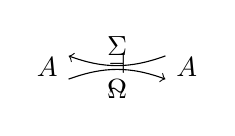
\begin{tikzpicture}[x=1.4em,y=1.4em]
  \node (L) at (0,0) {$A$};
  \node (R) at (3.6,0) {$A$};
  \draw[->] (3.05,0.3) to[bend left=20] node[above]{$\Sigma$} (0.55,0.3);
  \node at (1.8,0.1) {$\dashv$};
  \node at (1.8,-0.62) {$\scriptstyle\sim$};
  \draw[->] (0.55,-0.3) to[bend left=20] node[below]{$\Omega$} (3.05,-0.3);
\end{tikzpicture}
\end{center}
\end{proposition}

\begin{proof}
在命题 4.4.4 的证明中，\trAdjunction{} $\Sigma\dashv\Omega$ 被构造为诸%
\trAdjunction
\begin{center}
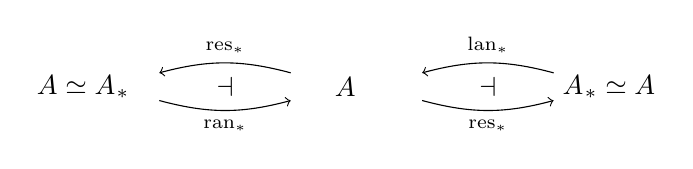
\begin{tikzpicture}[x=1.25em,y=1.25em]
  \node (p) at (0,0) {$A\simeq{\Alc}_{*}$};
  \node (q) at (7.6,0) {$\Asq$};
  \node (r) at (15.2,0) {${\Arc}_{*}\simeq A$};
  \draw[->] (6.0,0.4) to[bend right=15] node[above]{$\scriptstyle\mathrm{res}_{*}$} (2.2,0.4);
  \node at (4.1,0) {$\dashv$};
  \draw[->] (2.2,-0.4) to[bend right=15] node[below]{$\scriptstyle\mathrm{ran}_{*}$} (6.0,-0.4);
  \draw[->] (13.6,0.4) to[bend right=15] node[above]{$\scriptstyle\mathrm{lan}_{*}$} (9.8,0.4);
  \node at (11.7,0) {$\dashv$};
  \draw[->] (9.8,-0.4) to[bend right=15] node[below]{$\scriptstyle\mathrm{res}_{*}$} (13.6,-0.4);
\end{tikzpicture}
\end{center}
的复合，它们构造纤维序列与余纤维序列。由命题 2.1.9，这一复合\trAdjunction{}%
的单位与余单位由下给出
\begin{center}
\begin{tikzpicture}[x=1.25em,y=1.25em]
  \node (At) at (0,3.2) {$A$};
  \node (At2) at (8.4,3.2) {$A$};
  \node (ML) at (1.8,1.3) {${\Asq}_{*}$};
  \node (MR) at (6.6,1.3) {${\Asq}_{*}$};
  \node (Ab) at (4.2,-1.2) {$A$};
  \draw[double] (1.1,3.2) -- (7.3,3.2);
  \draw[double] (3.0,1.3) -- (5.4,1.3);
  \draw[->] (Ab) to[bend left=15] node[left]{$\mathrm{res}_{*}$} (ML);
  \draw[->] (Ab) to[bend right=15] node[right]{$\mathrm{ran}_{*}$} (MR);
  \draw[->] (ML) to[bend left=15] node[left]{$\mathrm{lan}_{*}$} (At);
  \draw[->] (MR) to[bend right=15] node[right]{$\mathrm{res}_{*}$} (At2);
  \node at (4.2,2.35) {$\scriptstyle\Downarrow\cong$};
  \node at (4.2,0.25) {$\scriptstyle\Downarrow\eta$};
  \draw[->] (At) to[bend right=35] node[left]{$\Sigma$} (Ab);
  \draw[->] (At2) to[bend left=35] node[right]{$\Omega$} (Ab);
  \node at (12.3,1.1) {与};
  \begin{scope}[shift={(14.6,0)}]
  \node (Bt) at (4.2,3.2) {$A$};
  \node (ML) at (1.8,1.3) {${\Asq}_{*}$};
  \node (MR) at (6.6,1.3) {${\Asq}_{*}$};
  \node (Bbl) at (0,-1.2) {$A$};
  \node (Bbr) at (8.4,-1.2) {$A$};
  \draw[double] (3.0,1.3) -- (5.4,1.3);
  \draw[double] (1.1,-1.2) -- (7.3,-1.2);
  \draw[->] (Bbl) to[bend left=15] node[left]{$\mathrm{ran}_{*}$} (ML);
  \draw[->] (Bbr) to[bend right=15] node[right]{$\mathrm{res}_{*}$} (MR);
  \draw[->] (ML) to[bend left=15] node[left]{$\mathrm{res}_{*}$} (Bt);
  \draw[->] (MR) to[bend right=15] node[right]{$\mathrm{lan}_{*}$} (Bt);
  \node at (4.2,2.35) {$\scriptstyle\Downarrow\epsilon$};
  \node at (4.2,0.25) {$\scriptstyle\Downarrow\cong$};
  \draw[->] (Bbl) to[bend right=35] node[left]{$\Omega$} (Bt);
  \draw[->] (Bt) to[bend right=35] node[right]{$\Sigma$} (Bbr);
  \end{scope}
\end{tikzpicture}
\end{center}
由定义 4.3.8，$\mathrm{res}_{*}\dashv\mathrm{ran}_{*}$ 的单位限制到\trPushout{}方块
的子对象上是一个同构。在一个\trStable{}\trInfinityCategory{}中，
$\mathrm{lan}_{*}\colon A\to{\Asq}_{*}$ 像中的余纤维序列都是\trPullback{}方块，
故这告诉我们 $\eta_{\mathrm{lan}_{*}}$ 是一个同构。对偶地，
$\mathrm{ran}_{*}\colon A\to{\Asq}_{*}$ 像中的纤维序列都是\trPushout{}方块，
这告诉我们 $\epsilon_{\mathrm{ran}_{*}}$ 是一个同构。于是，$\Sigma\dashv\Omega$
的单位与余单位可逆，故这些\trFunctor{}定义一个伴随\trEquivalence{}。
\end{proof}

刚才证明的这些结果提示了\trStable{}\trInfinityCategory{}的几个彼此%
\trEquivalence{}的刻画。条件 (iii) 的\trEquivalence{}归功于 Groth
\cite[\S3]{bib49}，后者在密切相关的稳定导子范畴（stable derivators）语境中
工作，并讨论了此处未提及的进一步等价条件。其余\trEquivalence{}由 Lurie 在
\cite{bib77}中建立。(iv)$\Rightarrow$(i) 的证明是对 Harpaz 的一个巧妙论证
（见 \cite[2.4]{bib51}）的改编。

\begin{theorem}[\trStable{}\trInfinityCategory{}的等价刻画]\label{thm:stable-characterizations}
在一个\trPointed{}\trInfinityCategory{} $A$ 中，下列条件彼此\trEquivalence{}，
且刻画了\textbf{\trStable{}\trInfinityCategory}：
\begin{itemize}
\item[(i)] $A$ 容许纤维与余纤维，且纤维序列与余纤维序列重合。
\item[(ii)] $A$ 容许\trPullback{}与\trPushout{}，且\trPullback{}方块与%
\trPushout{}方块重合。
\item[(iii)] $A$ 容许\trPullback{}与\trPushout{}，而且\trPullback\trFunctor{}
$\lim\colon\Alc\to A$ 保持\trPushout{}，同时\trPushout\trFunctor{}
$\colim\colon\Arc\to A$ 保持\trPullback{}。
\item[(iv)] $A$ 容许余纤维，且\trSuspension{}函子是一个\trEquivalence{}。
\item[(v)] $A$ 容许纤维，且\trLoops{}函子是一个\trEquivalence{}。
\end{itemize}
\end{theorem}

\begin{proof}
\cref{prop:pb-po-stable} 证明了 (i)$\Leftrightarrow$(ii)，而%
\cref{prop:loops-suspension-stable} 证明了 (i)$\Rightarrow$(iv) 与
(i)$\Rightarrow$(v)。故只剩下证明 (ii)$\Leftrightarrow$(iii) 以及这两条
蕴含的逆向，后者互为对偶。

设 (ii) 成立。我们可以应用\cref{lem:diagram-stable}看出图表∞-\trCategory{}
$\Alc$ 与 $\Arc$ 是稳定的。特别地，$\lim\colon\Alc\to A$ 与
$\colim\colon\Arc\to A$ 是\trStable{}\trInfinityCategory{}之间的\trFunctor{}，
据第 2 章中的定理 2.4.2，它们分别保持一切%
\trLimit{}与一切\trColimit{}。由于\trPushout{}方块与\trPullback{}方块重合，
我们看到\trPushout{}被\trPullback\trFunctor{}保持，而\trPullback{}被%
\trPushout\trFunctor{}保持，这就证明了 (iii)。

现在设 (iii) 成立。由练习 3.6.iv，说\trPushout\trFunctor{}保持\trPullback{}，
等价于说\trFunctor{} $\mathrm{lan}^{\lrcorner}\colon\Arc\to\Asq$ 保持%
\trPullback{}，亦即左侧的复合同构于右侧的绝对右\trLifting{}图：
\begin{center}
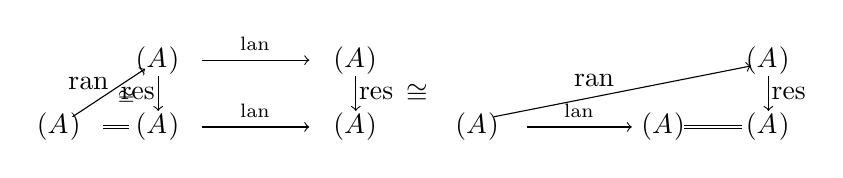
\begin{tikzpicture}[x=1.05em,y=1.05em]
  \node (tl) at (3.4,2.3) {$({\Arc})^{\square}$};
  \node (tr) at (10.2,2.3) {$({\Asq})^{\square}$};
  \node (bl1) at (0,0) {$({\Arc})^{\llcorner}$};
  \node (bl2) at (3.4,0) {$({\Arc})^{\llcorner}$};
  \node (br) at (10.2,0) {$({\Asq})^{\llcorner}$};
  \draw[->] (4.9,2.3) -- node[above]{$\scriptstyle\mathrm{lan}^{\square}$} (8.6,2.3);
  \draw[double] (1.5,0) -- (2.4,0);
  \draw[->] (4.9,0) -- node[above]{$\scriptstyle\mathrm{lan}^{\llcorner}$} (8.6,0);
  \draw[->] (3.4,1.75) -- (3.4,0.55);
  \node at (2.7,1.15) {$\mathrm{res}$};
  \draw[->] (10.2,1.75) -- (10.2,0.55);
  \node at (10.9,1.15) {$\mathrm{res}$};
  \draw[->] (0.45,0.35) -- (2.95,2.0);
  \node at (1.0,1.5) {$\mathrm{ran}$};
  \node at (2.3,1.0) {$\scriptstyle\cong$};
  \node at (12.3,1.15) {$\cong$};
  \begin{scope}[shift={(14.4,0)}]
  \node (bl) at (0,0) {$({\Arc})^{\llcorner}$};
  \node (br1) at (6.4,0) {$({\Asq})^{\llcorner}$};
  \node (br2) at (10.0,0) {$({\Asq})^{\llcorner}$};
  \node (trr) at (10.0,2.3) {$({\Asq})^{\square}$};
  \draw[->] (1.7,0) -- node[above]{$\scriptstyle\mathrm{lan}^{\llcorner}$} (5.3,0);
  \draw[double] (7.1,0) -- (9.1,0);
  \draw[->] (0.55,0.35) -- (9.4,2.1);
  \node at (4.0,1.6) {$\mathrm{ran}$};
  \draw[->] (10.0,1.75) -- (10.0,0.55);
  \node at (10.7,1.15) {$\mathrm{res}$};
  \end{scope}
\end{tikzpicture}
\end{center}
为看出 $A$ 中任何\trPullback{}方块也是\trPushout{}方块，考虑下方左图所描绘
的图表 $\psi\colon\Alc\to A^{\lrcorner\times\llcorner}$：它沿一个适当的%
\trFunctor{} $\lrcorner\times\llcorner\to\llcorner$ 作限制，把余跨度
$a\to c\leftarrow b$ 展开为一个由跨度构成的余跨度，该\trFunctor{}把五个元素
送到 $\llcorner$ 的终顶点、其余两个顶点各得两个元素。
\begin{center}
\begin{tikzpicture}[x=1.15em,y=1.15em]
  \node (b1) at (2.6,3.8) {$b$};
  \node (b2) at (5.8,3.5) {$b$};
  \node (c1) at (2.0,2.7) {$c$};
  \node (a1) at (-0.8,1.9) {$a$};
  \node (c2) at (2.0,1.9) {$c$};
  \node (c3) at (4.8,1.9) {$c$};
  \node (a2) at (-0.8,0.4) {$a$};
  \node (c4) at (2.0,0.4) {$c$};
  \node (c5) at (4.8,0.4) {$c$};
  \draw[->,dashed] (3.2,3.9) -- (5.1,3.6);
  \draw[->,dotted] (2.5,3.35) -- (2.1,3.05);
  \draw[->,dotted] (5.8,3.05) -- (4.9,2.35);
  \draw[->,dashed] (-0.2,1.9) -- (1.3,1.9);
  \draw[->,dotted] (2.6,1.9) -- (4.1,1.9);
  \draw[->,dotted] (2.0,2.45) -- (2.0,2.15);
  \draw[->,dotted] (-0.7,1.6) -- (-0.7,0.7);
  \draw[->,dotted] (2.0,1.6) -- (2.0,0.7);
  \draw[->,dotted] (4.8,1.6) -- (4.8,0.7);
  \draw[->,dotted] (-0.2,0.4) -- (1.3,0.4);
  \draw[->,dashed] (2.6,0.4) -- (4.1,0.4);
  \node at (8.2,1.9) {与};
  \begin{scope}[shift={(9.8,0.35)}]
  \node (B1) at (2.6,3.45) {$b$};
  \node (B2) at (6.2,3.15) {$b$};
  \node (C1) at (2.0,2.55) {$c$};
  \node (C6) at (6.6,2.2) {$c$};
  \node (A1) at (-0.8,1.55) {$a$};
  \node (C2) at (2.0,1.55) {$c$};
  \node (C3) at (4.6,1.55) {$c$};
  \node (C7) at (6.9,1.1) {$c$};
  \node (A2) at (-0.8,0.05) {$a$};
  \node (C4) at (2.0,0.05) {$c$};
  \node (C5) at (4.6,0.05) {$c$};
  \draw[->,dashed] (3.2,3.55) -- (5.5,3.25);
  \draw[->,dotted] (2.5,3.0) -- (2.1,2.85);
  \draw[->,dotted] (6.2,2.8) -- (4.9,2.0);
  \draw[->,dashed] (6.5,3.05) -- (6.55,2.5);
  \draw[->,dashed] (-0.2,1.55) -- (1.3,1.55);
  \draw[->,dashed] (2.6,1.55) -- (3.9,1.55);
  \draw[->,dashed] (5.2,1.5) -- (6.3,1.2);
  \draw[->,dotted] (2.0,2.3) -- (2.0,1.8);
  \draw[->,dotted] (-0.7,1.25) -- (-0.7,0.35);
  \draw[->,dotted] (2.0,1.25) -- (2.0,0.35);
  \draw[->,dotted] (4.6,1.25) -- (4.6,0.35);
  \draw[->,dotted] (6.75,1.85) -- (6.85,1.4);
  \draw[->,dashed] (-0.2,0.05) -- (1.3,0.05);
  \draw[->,dashed] (2.6,0.05) -- (3.9,0.05);
  \draw[->,dotted] (5.2,0.05) -- (6.2,0.05);
  \end{scope}
\end{tikzpicture}
\end{center}
由练习 2.3.iv，与 $\mathrm{lan}^{\lrcorner}\colon({\Arc})^{\llcorner}\to({\Asq})^{\llcorner}$
复合便得到上方右图，其中每个虚线方块都是\trPushout{}。由练习 4.3.i，
\trFunctor{} $\mathrm{ran}^{\square}\colon({\Asq})^{\llcorner}\to({\Asq})^{\square}$
自然同构于\trFunctor{}
$\mathrm{ran}^{\square}\colon({\Alc})^{\llcorner}\to({\Asq})^{\llcorner}$。
于是，与这一\trFunctor{}复合便作出诸点线余跨度的\trPullback{}，再由练习
2.3.iv 即得下方之图
\begin{center}
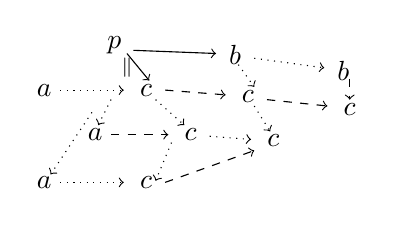
\begin{tikzpicture}[x=1.15em,y=1.15em]
  \node (p) at (1.6,4.2) {$p$};
  \node (b1) at (5.4,3.9) {$b$};
  \node (b2) at (8.8,3.4) {$b$};
  \node (a1) at (-0.6,2.8) {$a$};
  \node (c1) at (2.6,2.8) {$c$};
  \node (c2) at (5.8,2.6) {$c$};
  \node (c3) at (9.0,2.2) {$c$};
  \node (a2) at (1.0,1.4) {$a$};
  \node (c4) at (4.0,1.4) {$c$};
  \node (c5) at (6.6,1.2) {$c$};
  \node (a3) at (-0.6,-0.1) {$a$};
  \node (c6) at (2.6,-0.1) {$c$};
  \draw[->] (2.2,4.05) -- (4.8,3.95);
  \draw[->] (2.0,3.95) -- (2.7,3.1);
  \node at (2.0,3.5) {$\scriptstyle\Vert$};
  \draw[->,dotted] (6.0,3.8) -- (8.2,3.5);
  \draw[->,dotted] (5.5,3.6) -- (6.0,2.9);
  \draw[->,dashed] (9.0,3.15) -- (9.0,2.5);
  \draw[->,dotted] (-0.1,2.8) -- (1.9,2.8);
  \draw[->,dashed] (3.2,2.8) -- (5.1,2.65);
  \draw[->,dashed] (6.4,2.5) -- (8.3,2.3);
  \draw[->,dotted] (1.5,2.5) -- (1.1,1.7);
  \draw[->,dotted] (2.9,2.5) -- (3.8,1.7);
  \draw[->,dotted] (6.0,2.3) -- (6.5,1.5);
  \draw[->,dashed] (1.5,1.4) -- (3.3,1.4);
  \draw[->,dotted] (4.6,1.35) -- (5.9,1.25);
  \draw[->,dotted] (0.9,2.1) -- (-0.4,0.15);
  \draw[->,dotted] (3.4,1.15) -- (2.9,-0.05);
  \draw[->,dotted] (-0.1,-0.1) -- (1.9,-0.1);
  \draw[->,dashed] (3.2,-0.1) -- (6.0,0.9);
\end{tikzpicture}
\end{center}
其中 $p$ 是原余跨度 $a\to c\leftarrow b$ 的\trPullback{}。由于自然同构
$\mathrm{lan}^{\square}\circ\mathrm{ran}\cong\mathrm{ran}\circ\mathrm{lan}^{\lrcorner}$，
这张图也可以这样得到：先作诸点线跨度的\trPullback{}，再取每个余跨度的%
\trPushout{}。这样我们看到：上方左图的实线箭头\trPullback{}方块也是一个%
\trPushout{}。对偶构造完成了 (iii)$\Rightarrow$(ii) 的证明。

剩下要证明的是 (iv)$\Rightarrow$(i)。设 (iv) 成立，第一个任务是证明任何
余纤维序列 $d\colon D\to\Asq$ 也是一个纤维序列，也就是说，图表
\begin{center}
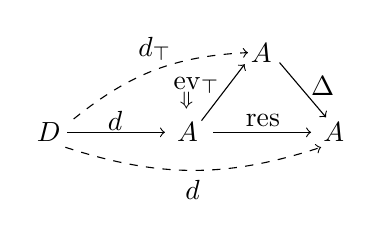
\begin{tikzpicture}[x=1.2em,y=1.2em]
  \node (D) at (0,0) {$D$};
  \node (A) at (6.4,2.4) {$A$};
  \node (Asq) at (4.2,0) {$\Asq$};
  \node (AL) at (8.6,0) {$\Alc$};
  \draw[->,dashed] (0.75,0.4) to[bend left=18] node[above]{$d_{\top}$} (6.0,2.4);
  \draw[->] (0.55,0) -- (3.5,0);
  \node at (2.0,0.35) {$d$};
  \draw[->] (4.95,0) -- (7.9,0);
  \node at (6.45,0.35) {$\mathrm{res}$};
  \draw[->] (4.6,0.35) -- (5.9,2.05);
  \node at (4.45,1.4) {$\mathrm{ev}_{\top}$};
  \node at (4.15,0.95) {$\scriptstyle\Downarrow$};
  \draw[->] (6.95,2.1) -- (8.35,0.45);
  \node at (8.25,1.4) {$\Delta$};
  \draw[->,dashed] (0.5,-0.45) to[bend right=18] node[below]{$d_{\llcorner}$} (8.2,-0.45);
\end{tikzpicture}
\end{center}
是绝对右提升的，其中该自然变换由\trFunctor{} $\llcorner\times 2\to\square$
诱导——后者定义了交换方块在其底余跨度之上的典范锥。由定理 3.5.3，为证此图
绝对右提升，只需证诱导映射定义一个纤维化\trEquivalence{}
$\mathrm{Hom}_A(A,d_{\top})\simeq_{D\times A}\mathrm{Hom}_{\Alc}(\Delta,d_{\llcorner})$。
由于 $\Sigma\colon A\simeq A$ 是一个\trEquivalence{}，由命题 3.4.5，下列余跨度
映射
\begin{center}
\begin{tikzpicture}[x=1.05em,y=1.05em]
  \node (Dt) at (0,2.2) {$D$};
  \node (Am) at (4.6,2.2) {$A$};
  \node (Ar) at (8.0,2.2) {$A$};
  \node (Db) at (0,0) {$D$};
  \node (Bm) at (4.6,0) {$A$};
  \node (Br) at (8.0,0) {$A$};
  \draw[double] (0,1.65) -- (0,0.55);
  \draw[->] (0.6,2.2) -- node[above]{$d_{\top}$} (3.8,2.2);
  \draw[double] (5.4,2.2) -- (7.3,2.2);
  \draw[double] (8.0,1.65) -- (8.0,0.55);
  \draw[->] (4.6,1.65) -- node[left]{$\Sigma$} (4.6,0.55);
  \node at (5.35,1.1) {$\scriptstyle\Downarrow\Sigma$};
  \draw[->] (0.6,0) -- node[below]{$\Sigma d_{\top}$} (3.8,0);
  \draw[->] (7.4,0) -- node[below]{$\Sigma$} (5.4,0);
  \node at (9.8,1.1) {与};
  \begin{scope}[shift={(11.6,0)}]
  \node (Dt) at (0,2.2) {$D$};
  \node (Am) at (5.2,2.2) {$\Alc$};
  \node (Ar) at (9.4,2.2) {$A$};
  \node (Db) at (0,0) {$D$};
  \node (Bm) at (5.2,0) {$\Alc$};
  \node (Br) at (9.4,0) {$A$};
  \draw[double] (0,1.65) -- (0,0.55);
  \draw[->] (0.6,2.2) -- node[above]{$d_{\llcorner}$} (4.4,2.2);
  \draw[->] (7.2,2.2) -- node[above]{$\Delta$} (6.0,2.2);
  \draw[double] (9.4,1.65) -- (9.4,0.55);
  \draw[->] (5.2,1.65) -- node[left]{$\Sigma^{\llcorner}$} (5.2,0.55);
  \node at (6.1,1.1) {$\scriptstyle\Downarrow\Sigma^{\llcorner}$};
  \draw[->] (0.6,0) -- node[below]{$\Sigma d_{\llcorner}$} (4.4,0);
  \draw[->] (8.8,0) -- node[below]{$\Delta\Sigma$} (6.0,0);
  \end{scope}
\end{tikzpicture}
\end{center}
诱导出 $D\times A$ 之上的逗号∞-\trCategory{}的\trEquivalence{}，于下方垂直
展示：
\begin{center}
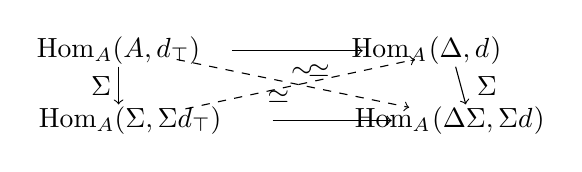
\begin{tikzpicture}[x=1.05em,y=1.05em]
  \node (TL) at (0,2.4) {$\mathrm{Hom}_A(A,d_{\top})$};
  \node (TR) at (10.6,2.4) {$\mathrm{Hom}_{\Alc}(\Delta,d_{\llcorner})$};
  \node (BL) at (0.4,0) {$\mathrm{Hom}_A(\Sigma,\Sigma d_{\top})$};
  \node (BR) at (11.4,0) {$\mathrm{Hom}_{\Alc}(\Delta\Sigma,\Sigma d_{\llcorner})$};
  \draw[->] (3.9,2.4) -- (8.4,2.4);
  \draw[->] (5.3,0) -- (9.4,0);
  \draw[->] (0,1.85) -- (0,0.55);
  \node at (-0.6,1.2) {$\Sigma$};
  \draw[->] (11.6,1.85) -- (11.95,0.55);
  \node at (12.7,1.2) {$\Sigma^{\llcorner}$};
  \draw[->,dashed] (2.0,2.1) -- (10.0,0.45);
  \node at (6.6,1.7) {$\sim\!\simeq$};
  \draw[->,dashed] (2.3,0.4) -- (10.2,2.1);
  \node at (5.5,0.8) {$\simeq$};
\end{tikzpicture}
\end{center}
我们的任务是定义那条虚线对角态射，使得我们可以应用命题 3.4.11 论证该图表在
纤维化同构意义下交换。由∞-\trInfinityCosmos{}中\trEquivalence{}的%
\trTwoOfSixProperty{}（见注 1.2.21 与练习 1.4.iii），
由此推出上水平映射定义一个纤维化\trEquivalence{}，见证余纤维序列也是纤维序列
这一事实。

为解释这一构造，给余纤维序列 $d\colon D\to\Asq$ 中的诸广义元素起些名字是有
帮助的，如下方左图所描绘：
\begin{center}
\begin{tikzpicture}[x=1.3em,y=1.3em]
  \node (a) at (0,2.2) {$a$};
  \node (b) at (4.4,2.2) {$b$};
  \node (st) at (8.4,2.2) {$*$};
  \node (st2) at (0,0) {$*$};
  \node (c) at (4.4,0) {$c$};
  \node (sa) at (9.2,0) {$\Sigma a$};
  \draw[->] (0.55,2.2) -- (3.7,2.2);
  \draw[->] (5.0,2.2) -- (7.7,2.2);
  \draw[->] (0,1.65) -- (0,0.55);
  \draw[->] (4.4,1.65) -- (4.4,0.55);
  \node at (3.75,1.25) {$\scriptstyle\ulcorner$};
  \draw[->,dashed] (8.6,1.7) -- (9.15,0.55);
  \node at (7.8,1.25) {$\scriptstyle\ulcorner$};
  \draw[->] (0.55,0) -- (3.7,0);
  \draw[->,dashed] (5.1,0) -- (8.4,0);
\end{tikzpicture}
\end{center}
这里 $a\colon D\to A$ 表示广义元素 $d_{\top}$。由于余纤维序列
$a\to b\to c$ 定义一个\trPushout{}方块，当我们限制到其右边 $b\to c$ 并作
余纤维时，所得\trElement{}由命题 4.3.11 同构于\trSuspension $\Sigma a$。特别地，
我们有如下形式的绝对左\trLifting{}图：
\begin{center}
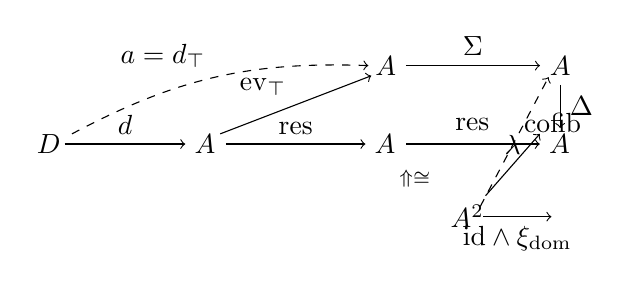
\begin{tikzpicture}[x=1.05em,y=1.05em]
  \node (D) at (0,0) {$D$};
  \node (Asq) at (5.4,0) {$\Asq$};
  \node (AL) at (11.6,0) {$\Alc$};
  \node (AR) at (17.6,0) {$\Arc$};
  \node (A1) at (11.6,2.7) {$A$};
  \node (A2) at (17.6,2.7) {$A$};
  \node (A2n) at (14.4,-2.5) {$A^{2}$};
  \draw[->,dashed] (0.8,0.35) to[bend left=15] node[above left]{$a=d_{\top}$} (11.0,2.7);
  \draw[->] (A1) -- node[above]{$\Sigma$} (A2);
  \draw[->] (5.9,0.35) -- node[above left]{$\mathrm{ev}_{\top}$} (11.1,2.35);
  \draw[->] (A2) -- node[right]{$\Delta$} (17.6,0.55);
  \draw[->] (0.55,0) -- node[above]{$d$} (4.7,0);
  \draw[->] (6.1,0) -- node[above]{$\mathrm{res}$} (10.9,0);
  \draw[->] (12.3,0) -- node[above]{$\mathrm{res}_{\lrcorner}$} (16.9,0);
  \draw[->,dashed] (14.85,-2.15) -- node[above right]{$\mathrm{cofib}$} (17.2,2.3);
  \draw[->] (A2n) -- node[above]{$\qcor{\lambda}$} (16.9,0.35);
  \draw[->] (14.95,-2.5) -- node[below]{$\mathrm{id}\wedge\qcor{\xi_{\mathrm{dom}}}$} (17.3,-2.5);
  \node at (12.6,-1.2) {$\scriptstyle\Uparrow\cong$};
\end{tikzpicture}
\end{center}
其自然变换分量由一个\trFunctor{} $\qcor{\lambda}$ 表示；为供后用，我们把它
限制到 $d_{\llcorner}$ 之上的锥∞-\trCategory{}：
\begin{center}
\begin{tikzpicture}[x=1.05em,y=1.05em]
  \node (Hom) at (0,1.1) {$\mathrm{Hom}_{\Alc}(\Delta,d_{\llcorner})$};
  \node (D) at (7.0,1.1) {$D$};
  \node (A12) at (14.6,1.1) {$A^{\lrcorner\times 2}$};
  \draw[->] (4.6,1.1) -- node[above]{$p_{1}$} (5.9,1.1);
  \draw[->] (8.1,1.1) -- node[above]{$\qcor{\lambda}$} (12.8,1.1);
  \node at (17.6,1.1) {，};
  \begin{scope}[shift={(19.0,0)}]
  \node (c) at (0,2.2) {$c$};
  \node (b) at (4.0,2.2) {$b$};
  \node (st) at (8.0,2.2) {$*$};
  \node (sa1) at (0,0) {$\Sigma a$};
  \node (sa2) at (4.0,0) {$\Sigma a$};
  \node (sa3) at (8.0,0) {$\Sigma a$};
  \draw[->] (3.4,2.2) -- (1.3,2.2);
  \draw[->] (4.6,2.2) -- (7.3,2.2);
  \draw[->] (0,1.65) -- (0,0.55);
  \draw[->] (4.0,1.65) -- (4.0,0.55);
  \draw[->] (8.0,1.65) -- (8.0,0.55);
  \draw[double] (1.3,0) -- (2.7,0);
  \draw[double] (5.3,0) -- (6.7,0);
  \end{scope}
\end{tikzpicture}
\end{center}
由命题 4.2.7，逗号∞-\trCategory{}
$\mathrm{Hom}_{\Alc}(\Delta,d_{\llcorner})$ \trEquivalence{}于\trPullback
\begin{center}
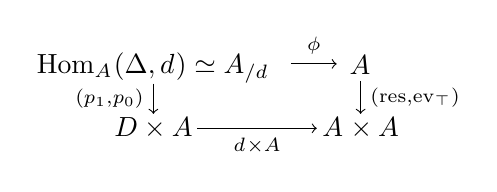
\begin{tikzpicture}[x=0.72em,y=0.95em]
  \node (TL) at (0,2.3) {$\mathrm{Hom}_{\Alc}(\Delta,d_{\llcorner})\simeq A_{/d_{\llcorner}}$};
  \node (TR) at (10.4,2.4) {$\Asq$};
  \node (BL) at (0,0) {$D\times A$};
  \node (BR) at (10.4,0) {$\Alc\times A$};
  \draw[->] (6.9,2.45) -- node[above]{$\scriptstyle\qcor{\phi}$} (9.2,2.45);
  \node at (7.6,1.55) {$\scriptstyle\lrcorner$};
  \draw[->] (0,1.7) -- node[left]{$\scriptstyle(p_{1},p_{0})$} (0,0.55);
  \draw[->] (10.4,1.8) -- node[right]{$\scriptstyle(\mathrm{res},\mathrm{ev}_{\top})$} (10.4,0.55);
  \draw[->] (2.2,0) -- node[below]{$\scriptstyle d_{\llcorner}\times A$} (8.2,0);
\end{tikzpicture}
\end{center}
这里 $\qcor{\phi}$ 定义一个方块，如下方左图所示，其中
$z\colon\mathrm{Hom}_{\Alc}(\Delta,d_{\llcorner})\to A$ 表示广义元素
$p_0\colon\mathrm{Hom}_{\Alc}(\Delta,d_{\llcorner})\Rightarrow A$——它投影为
$d_{\llcorner}$ 之上一个锥的顶点：
\begin{center}
\begin{tikzpicture}[x=1.3em,y=1.3em]
  \node (st) at (0,2.2) {$*$};
  \node (z) at (4.2,2.2) {$z$};
  \node (c) at (0,0) {$c$};
  \node (b) at (4.2,0) {$b$};
  \draw[->] (3.5,2.2) -- (1.1,2.2);
  \draw[->] (0,1.65) -- (0,0.55);
  \draw[->] (4.2,1.65) -- (4.2,0.55);
  \draw[->] (3.5,0) -- (1.1,0);
  \node at (2.6,1.25) {$\scriptstyle\lrcorner$};
  \node at (7.0,1.1) {与};
  \begin{scope}[shift={(8.8,0)}]
  \node (st1) at (0,2.2) {$*$};
  \node (z2) at (4.2,2.2) {$z$};
  \node (st2) at (8.4,2.2) {$*$};
  \node (c2) at (0,0) {$c$};
  \node (b2) at (4.2,0) {$b$};
  \node (st3) at (8.4,0) {$*$};
  \draw[->] (3.5,2.2) -- (1.1,2.2);
  \draw[->] (4.9,2.2) -- (7.7,2.2);
  \draw[->] (0,1.65) -- (0,0.55);
  \draw[->] (4.2,1.65) -- (4.2,0.55);
  \draw[->] (8.4,1.65) -- (8.4,0.55);
  \draw[->] (3.5,0) -- (1.1,0);
  \draw[->] (4.9,0) -- (7.7,0);
  \end{scope}
\end{tikzpicture}
\end{center}
这一方块可以沿着由余点\trFunctor{}所定义的方块粘合，从而扩展为上方右图的
跨度映射：
\begin{center}
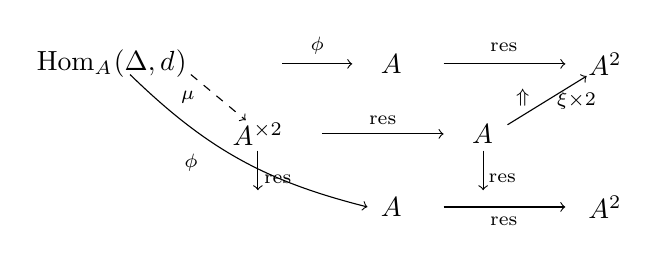
\begin{tikzpicture}[x=1.1em,y=1.1em]
  \node (Hom) at (0,3.6) {$\mathrm{Hom}_{\Alc}(\Delta,d_{\llcorner})$};
  \node (Asq1) at (9.2,3.6) {$\Asq$};
  \node (A21) at (16.2,3.6) {$A^{2}$};
  \node (Arc2) at (4.8,1.3) {$A^{\lrcorner\times 2}$};
  \node (Asq2) at (12.2,1.3) {$\Asq$};
  \node (Asq3) at (9.2,-1.1) {$\Asq$};
  \node (A22) at (16.2,-1.1) {$A^{2}$};
  \draw[->] (5.6,3.6) -- node[above]{$\scriptstyle\qcor{\phi}$} (7.9,3.6);
  \draw[->] (10.9,3.6) -- node[above]{$\scriptstyle\mathrm{res}_{\lrcorner}$} (14.9,3.6);
  \draw[->,dashed] (2.6,3.25) -- (4.4,1.75);
  \node at (2.5,2.5) {$\scriptstyle\qcor{\mu}$};
  \draw[->] (6.9,1.3) -- node[above]{$\scriptstyle\mathrm{res}$} (10.9,1.3);
  \node at (9.9,2.35) {$\scriptstyle\lrcorner$};
  \draw[->] (4.8,0.75) -- (4.8,-0.55);
  \node at (5.45,-0.2) {$\scriptstyle\mathrm{res}$};
  \draw[->] (12.2,0.75) -- (12.2,-0.55);
  \node at (12.85,-0.2) {$\scriptstyle\mathrm{res}_{\lrcorner}$};
  \draw[->] (10.9,-1.1) -- node[below]{$\scriptstyle\mathrm{res}_{\lrcorner}$} (14.9,-1.1);
  \draw[->] (0.6,3.25) to[bend right=15] (8.4,-1.1);
  \node at (2.6,0.35) {$\scriptstyle\qcor{\phi}$};
  \draw[->] (13.0,1.6) -- node[right]{$\scriptstyle\qcor{\xi}\times 2$} (15.6,3.2);
  \node at (13.5,2.5) {$\scriptstyle\Uparrow$};
\end{tikzpicture}
\end{center}
图表 $\qcor{\mu}$ 与 $\qcor{\lambda}$ 粘合在一起，构成一个图表
$\mathrm{Hom}_{\Alc}(\Delta,d_{\llcorner})\to A^{\lrcorner\times 3}$，如下
\begin{center}
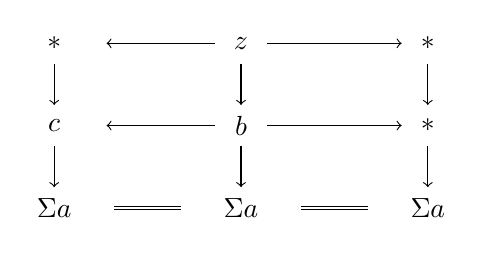
\begin{tikzpicture}[x=1.35em,y=1.35em]
  \node (r1c1) at (0,4.4) {$*$};
  \node (r1c2) at (5.0,4.4) {$z$};
  \node (r1c3) at (10.0,4.4) {$*$};
  \node (r2c1) at (0,2.2) {$c$};
  \node (r2c2) at (5.0,2.2) {$b$};
  \node (r2c3) at (10.0,2.2) {$*$};
  \node (r3c1) at (0,0) {$\Sigma a$};
  \node (r3c2) at (5.0,0) {$\Sigma a$};
  \node (r3c3) at (10.0,0) {$\Sigma a$};
  \draw[->] (4.3,4.4) -- (1.4,4.4);
  \draw[->] (5.7,4.4) -- (9.3,4.4);
  \draw[->] (0,3.85) -- (0,2.75);
  \draw[->] (5.0,3.85) -- (5.0,2.75);
  \draw[->] (10.0,3.85) -- (10.0,2.75);
  \draw[->] (4.3,2.2) -- (1.4,2.2);
  \draw[->] (5.7,2.2) -- (9.3,2.2);
  \draw[->] (0,1.65) -- (0,0.55);
  \draw[->] (5.0,1.65) -- (5.0,0.55);
  \draw[->] (10.0,1.65) -- (10.0,0.55);
  \draw[double] (1.6,0) -- (3.4,0);
  \draw[double] (6.6,0) -- (8.4,0);
\end{tikzpicture}
\end{center}
由此我们提取出一个余跨度映射的复合，它定义下方左图的自然变换：
\begin{center}
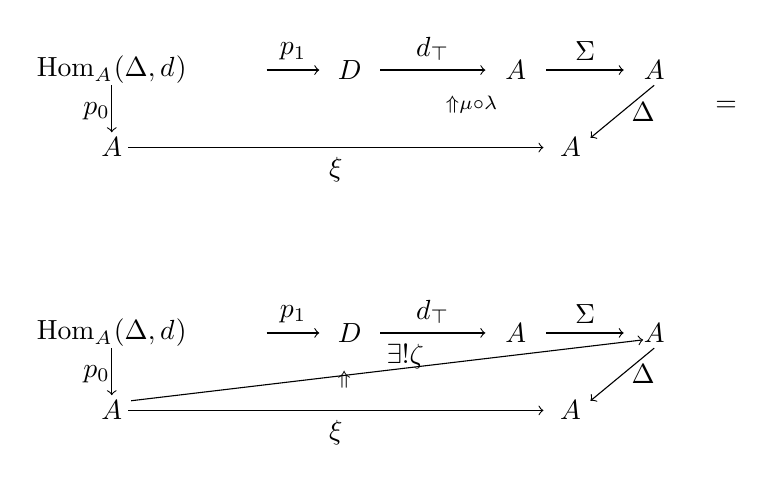
\begin{tikzpicture}[x=1.0em,y=1.0em]
  \node (Hom) at (0,2.4) {$\mathrm{Hom}_{\Alc}(\Delta,d_{\llcorner})$};
  \node (D) at (8.6,2.4) {$D$};
  \node (A1) at (14.6,2.4) {$A$};
  \node (A2) at (19.6,2.4) {$A$};
  \node (A0) at (0,-0.4) {$A$};
  \node (AR) at (16.6,-0.4) {$\Arc$};
  \draw[->] (5.6,2.4) -- node[above]{$p_{1}$} (7.5,2.4);
  \draw[->] (9.7,2.4) -- node[above]{$d_{\top}$} (13.5,2.4);
  \draw[->] (15.7,2.4) -- node[above]{$\Sigma$} (18.5,2.4);
  \draw[->] (0,1.85) -- (0,0.15);
  \node at (-0.55,0.9) {$p_{0}$};
  \draw[->] (19.6,1.85) -- (17.3,-0.05);
  \node at (19.2,0.9) {$\Delta$};
  \draw[->] (0.6,-0.4) -- node[below]{$\xi$} (15.6,-0.4);
  \node at (13.0,1.15) {$\scriptstyle\Uparrow\mu\circ\lambda$};
  \node at (22.2,1.1) {$=$};
  \begin{scope}[shift={(0,-9.5)}]
  \node (Hom) at (0,2.4) {$\mathrm{Hom}_{\Alc}(\Delta,d_{\llcorner})$};
  \node (D) at (8.6,2.4) {$D$};
  \node (A1) at (14.6,2.4) {$A$};
  \node (A2) at (19.6,2.4) {$A$};
  \node (A0) at (0,-0.4) {$A$};
  \node (AR) at (16.6,-0.4) {$\Arc$};
  \draw[->] (5.6,2.4) -- node[above]{$p_{1}$} (7.5,2.4);
  \draw[->] (9.7,2.4) -- node[above]{$d_{\top}$} (13.5,2.4);
  \draw[->] (15.7,2.4) -- node[above]{$\Sigma$} (18.5,2.4);
  \draw[->] (0,1.85) -- (0,0.15);
  \node at (-0.55,0.9) {$p_{0}$};
  \draw[->] (19.6,1.85) -- (17.3,-0.05);
  \node at (19.2,0.9) {$\Delta$};
  \draw[->] (0.6,-0.4) -- node[below]{$\xi$} (15.6,-0.4);
  \draw[->] (0.7,-0.05) -- (19.2,2.15);
  \node at (10.6,1.55) {$\exists!\qcor{\zeta}$};
  \node at (8.4,0.7) {$\scriptstyle\Uparrow$};
  \end{scope}
\end{tikzpicture}
\end{center}
这可经由\cref{def:loops-and-suspension}的绝对左\trLifting{}图分解，从而定义
一个自然变换 $\zeta$。由\trOneCellInduction{}，$\zeta$ 定义所求的\trFunctor{}
$\qcor{\zeta}\colon\mathrm{Hom}_{\Alc}(\Delta,d_{\llcorner})\to\mathrm{Hom}_A(\Sigma,\Sigma d_{\top})$（于 $D\times A$ 之上），
这就完成了「余纤维序列 $a\to b\to c$ 也是纤维序列」的证明。

现在为证明每个箭头 $f\colon a\to b$ 都容许纤维，先作其余纤维。由于 $\Sigma$
是一个\trEquivalence{}，存在 $A$ 的某个\trElement{} $k$ 使得
$\mathrm{cofib}(f)\cong\Sigma k$。由刚才证明的结论，余纤维序列
$a\to b\to\Sigma k$ 与 $k\to *\to\Sigma k$ 都是纤维序列，特别地，下方右手边
的方块既是\trPushout{}又是\trPullback{}：
\begin{center}
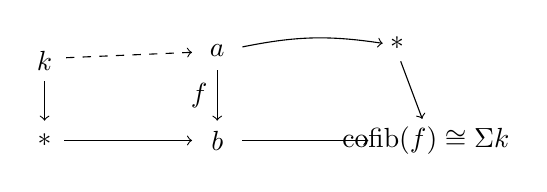
\begin{tikzpicture}[x=1.3em,y=1.3em]
  \node (k) at (0,2.2) {$k$};
  \node (a) at (4.8,2.5) {$a$};
  \node (st) at (9.8,2.7) {$*$};
  \node (st2) at (0,0) {$*$};
  \node (b) at (4.8,0) {$b$};
  \node (cf) at (10.6,0) {$\mathrm{cofib}(f)\cong\Sigma k$};
  \draw[->,dashed] (0.6,2.3) -- (4.1,2.45);
  \draw[->] (5.5,2.6) to[bend left=10] (9.4,2.7);
  \draw[->] (0,1.65) -- (0,0.55);
  \draw[->] (4.8,1.95) -- (4.8,0.55);
  \node at (4.3,1.25) {$f$};
  \draw[->] (9.9,2.2) -- (10.5,0.6);
  \draw[->] (0.55,0) -- (4.1,0);
  \draw[->] (5.5,0) -- (9.0,0);
  \node at (2.4,1.25) {$\scriptstyle\lrcorner$};
  \node at (7.5,1.35) {$\scriptstyle\ulcorner$};
\end{tikzpicture}
\end{center}
于是，外矩形可经过右手边的方块分解，而这个复合矩形——它作为\trPushout{}给出
——也是一个\trPullback{}。再由拉回消去，左手边的方块是一个\trPullback{}，它定义
$f\colon a\to b$ 的纤维 $k\cong\mathrm{fib}(f)$。

为看出纤维序列 $k\to a\to b$ 也是余纤维序列，作余纤维序列 $k\to a\to c$。
我们的任务是证明：从
下方左图立方的前面向其背面的映射是一个同构：
\begin{center}
\begin{tikzpicture}[x=1.25em,y=1.25em]
  \node (kb) at (2.9,3.3) {$k$};
  \node (ab) at (7.7,3.3) {$a$};
  \node (kf) at (0,2.0) {$k$};
  \node (af) at (4.8,2.0) {$a$};
  \node (sb) at (2.9,0.9) {$*$};
  \node (cb) at (7.7,0.9) {$c$};
  \node (sf) at (0,-0.4) {$*$};
  \node (bf) at (4.8,-0.4) {$b$};
  \draw[->] (kb) -- (ab);
  \draw[->] (kf) -- (af);
  \draw[->] (sb) -- (cb);
  \draw[->] (sf) -- (bf);
  \draw[->] (kf) -- (kb);
  \draw[->] (af) -- (ab);
  \draw[->] (sf) -- (sb);
  \draw[->] (bf) -- (cb);
  \draw[->] (kf) -- (sf);
  \draw[->] (af) -- (bf);
  \node at (1.7,2.75) {$\scriptstyle\Vert$};
  \node at (3.7,1.75) {$\scriptstyle\Vert$};
  \node at (6.0,2.8) {$\scriptstyle\lrcorner$};
  \node at (6.3,0.35) {$\scriptstyle\ulcorner$};
  \node at (5.4,1.25) {$\scriptstyle\Vert$};
  \node at (10.6,1.3) {与};
  \begin{scope}[shift={(12.4,0)}]
  \node (zb) at (2.9,4.4) {$z$};
  \node (stb1) at (7.7,4.4) {$*$};
  \node (wf) at (0,3.1) {$w$};
  \node (stf1) at (4.8,3.1) {$*$};
  \node (kb) at (2.9,1.7) {$k$};
  \node (ab) at (7.7,1.7) {$a$};
  \node (kf) at (0,0.4) {$k$};
  \node (af) at (4.8,0.4) {$a$};
  \node (sb) at (2.9,-1.0) {$*$};
  \node (cb) at (7.7,-1.0) {$c$};
  \node (sf) at (0,-2.3) {$*$};
  \node (bf) at (4.8,-2.3) {$b$};
  \draw[->] (zb) -- (stb1);
  \draw[->,dashed] (wf) -- (stf1);
  \draw[->] (kb) -- (ab);
  \draw[->] (kf) -- (af);
  \draw[->] (sb) -- (cb);
  \draw[->] (sf) -- (bf);
  \draw[->,dashed] (zb) -- (wf);
  \node at (1.4,4.0) {$e$};
  \draw[->] (zb) -- (kb);
  \draw[->] (stb1) -- (ab);
  \draw[->] (wf) -- (kf);
  \draw[->] (stf1) -- (af);
  \draw[->] (kb) -- (sb);
  \draw[->] (ab) -- (cb);
  \draw[->] (kf) -- (sf);
  \draw[->,dashed] (af) -- (bf);
  \draw[->] (stf1) -- (stb1);
  \draw[->] (kf) -- (kb);
  \draw[->] (af) -- (ab);
  \draw[->] (sf) -- (sb);
  \draw[->,dashed] (cb) -- (bf);
  \node at (1.6,2.55) {$\scriptstyle\Vert$};
  \node at (3.8,1.15) {$\scriptstyle\Vert$};
  \node at (6.1,2.2) {$\scriptstyle\Vert$};
  \node at (5.9,3.75) {$\scriptstyle\lrcorner$};
  \node at (6.2,0.9) {$\scriptstyle\ulcorner$};
  \node at (6.0,-1.85) {$\scriptstyle\Vert$};
  \end{scope}
\end{tikzpicture}
\end{center}
由于 $\Sigma$ 是一个\trEquivalence{}，存在 $A$ 中的箭头 $e\colon z\to w$，其在
$\Sigma$ 下的像同构于诱导映射 $c\to b$。余纤维序列 $z\to *\to c$ 与
$w\to *\to b$ 也是纤维序列，故由拉回消去我们看到：上左棱柱中被诱导的上前
方块与上背方块都是\trPullback{}。由此我们看出 $e\colon z\to w$ 是 $k\to a$
的两个纤维之间的映射。于是 $e$ 是一个同构，而同构
$c\cong\Sigma z\cong\Sigma w\cong b$ 揭示：原纤维序列 $k\to a\to b$ 也是一个
余纤维序列。
\end{proof}

\begin{remark}\label{rem:finite-limits-stable}
事实上，\trStable{}\trInfinityCategory{}拥有一切有限\trLimit{}与有限%
\trColimit{}，意即由只含有限多个非退化\trSimplex{}的\trSimplicialSet{}作索引的%
\trLimit{}与\trColimit{}。更一般地，任何带\trPullback{}与一个\trTerminal{}元素
的∞-\trCategory{}容许一切有限\trLimit{}，后者可以沿\trSimplicialSet{}的维数
归纳地定义（见 \cite[4.4.2.4]{bib78}、\cite[6.3.9]{bib112}）。由这一构造与
\cref{thm:stable-characterizations} 的条件 (iii) 可推出：在一个%
\trStable{}\trInfinityCategory{}中，对任何有限图表形状的\trLimit\trFunctor{}%
与\trColimit\trFunctor{}保持一切有限余极限与一切有限极限。
\end{remark}

\begin{definition}\label{def:binary-direct-sums}
一个\trPointed{}\trInfinityCategory{} $A$ 容许\textbf{二元直和}（binary
direct sums），如果存在一个二函子
$\oplus\colon A\times A\to A$，它同时定义二元\trProduct{}与二元\trCoproduct{}，
使得余极限锥与极限锥的腿
\begin{center}
\begin{tikzpicture}[x=1.2em,y=1.2em]
  \node (AA1) at (0,0) {$A\times A$};
  \node (A1) at (4.4,2.2) {$A$};
  \node (AA2) at (8.0,0) {$A\times A$};
  \draw[->] (0.6,0.35) -- (3.9,1.95);
  \node at (1.9,1.35) {$\oplus$};
  \node at (3.0,0.95) {$\scriptstyle\Uparrow(\iota_{1},\iota_{2})$};
  \draw[->] (4.4,1.65) -- (4.4,0.5);
  \node at (4.95,1.1) {$\Delta$};
  \draw[double] (1.3,0) -- (6.4,0);
  \node at (10.9,1.1) {与};
  \begin{scope}[shift={(12.6,0)}]
  \node (BB1) at (0,0) {$A\times A$};
  \node (B1) at (4.4,2.2) {$A$};
  \node (BB2) at (8.0,0) {$A\times A$};
  \draw[->] (0.6,0.35) -- (3.9,1.95);
  \node at (1.9,1.35) {$\oplus$};
  \node at (3.1,0.9) {$\scriptstyle\Downarrow(\rho_{1},\rho_{2})$};
  \draw[->] (4.4,1.65) -- (4.4,0.5);
  \node at (4.95,1.1) {$\Delta$};
  \draw[double] (1.3,0) -- (6.4,0);
  \end{scope}
\end{tikzpicture}
\end{center}
满足下列涉及零映射的关系（见\cref{ex:zero-map}）：
$\rho_{1}\circ\iota_{1}=\mathrm{id}$、$\rho_{1}\circ\iota_{2}=0$、
$\rho_{2}\circ\iota_{1}=0$ 与 $\rho_{2}\circ\iota_{2}=\mathrm{id}$。
\end{definition}

\begin{lemma}\label{lem:stable-finite-direct-sums}
\emph{\trStable{}\trInfinityCategory{}容许有限直和。}
\end{lemma}

\begin{proof}
我们论证一个\trStable{}\trInfinityCategory{} $A$ 拥有二元直和，并留待%
\cref{ex:finite-direct-sums} 去扩充练习 2.3.i，以证明 $A$ 拥有有限直和。
直和二函子可以定义为零元素之上的一个\trPullback{}：
\begin{center}
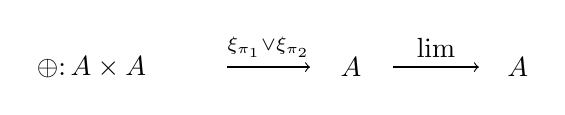
\begin{tikzpicture}[x=1.0em,y=1.0em]
  \node (a) at (0,0) {$\oplus\colon A\times A$};
  \node (b) at (9.4,0) {$\Alc$};
  \node (c) at (15.4,0) {$A$};
  \draw[->] (4.9,0) -- node[above]{$\scriptstyle\qcor{\xi_{\pi_{1}}}\vee\qcor{\xi_{\pi_{2}}}$} (7.9,0);
  \draw[->] (10.9,0) -- node[above]{$\lim$} (14.0,0);
\end{tikzpicture}
\end{center}
由练习 4.3.vii，这一构造保证直和是\trProduct{}。
为看出直和也是\trCoproduct{}，考虑图表 $A\times A\to\Asq$，其在广义元素
$(a,b)\colon X\to A\times A$ 处的像描绘如下：
\begin{center}
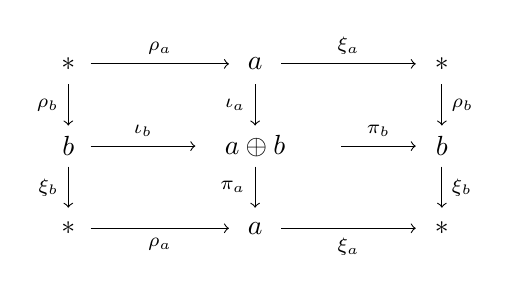
\begin{tikzpicture}[x=1.35em,y=1.35em]
  \node (r1c1) at (0,4.4) {$*$};
  \node (r1c2) at (5.0,4.4) {$a$};
  \node (r1c3) at (10.0,4.4) {$*$};
  \node (r2c1) at (0,2.2) {$b$};
  \node (r2c2) at (5.0,2.2) {$a\oplus b$};
  \node (r2c3) at (10.0,2.2) {$b$};
  \node (r3c1) at (0,0) {$*$};
  \node (r3c2) at (5.0,0) {$a$};
  \node (r3c3) at (10.0,0) {$*$};
  \draw[->] (0.6,4.4) -- node[above]{$\scriptstyle\qcor{\rho_{a}}$} (4.3,4.4);
  \draw[->] (5.7,4.4) -- node[above]{$\scriptstyle\qcor{\xi_{a}}$} (9.3,4.4);
  \draw[->] (0,3.85) -- node[left]{$\scriptstyle\qcor{\rho_{b}}$} (0,2.75);
  \draw[->] (5.0,3.85) -- node[left]{$\scriptstyle\iota_{a}$} (5.0,2.75);
  \draw[->] (10.0,3.85) -- node[right]{$\scriptstyle\qcor{\rho_{b}}$} (10.0,2.75);
  \node at (2.6,3.3) {$\scriptstyle\lrcorner$};
  \node at (7.5,3.3) {$\scriptstyle\lrcorner$};
  \draw[->] (0.6,2.2) -- node[above]{$\scriptstyle\iota_{b}$} (3.4,2.2);
  \draw[->] (7.3,2.2) -- node[above]{$\scriptstyle\pi_{b}$} (9.3,2.2);
  \draw[->] (0,1.65) -- node[left]{$\scriptstyle\qcor{\xi_{b}}$} (0,0.55);
  \draw[->] (5.0,1.65) -- node[left]{$\scriptstyle\pi_{a}$} (5.0,0.55);
  \draw[->] (10.0,1.65) -- node[right]{$\scriptstyle\qcor{\xi_{b}}$} (10.0,0.55);
  \node at (2.6,1.1) {$\scriptstyle\lrcorner$};
  \node at (7.5,1.1) {$\scriptstyle\lrcorner$};
  \draw[->] (0.6,0) -- node[below]{$\scriptstyle\qcor{\rho_{a}}$} (4.3,0);
  \draw[->] (5.7,0) -- node[below]{$\scriptstyle\qcor{\xi_{a}}$} (9.3,0);
\end{tikzpicture}
\end{center}
这里诸垂直与水平复合态射都是恒等，而右手边的矩形与下方矩形由沿一个投影%
\trFunctor{} $2\times 2\to 2$ 作限制而定义，随后再用右下方\trPullback{}的%
\trUniversalProperty{}分解到该方块上。由练习 2.3.iv，这些矩形各自自身都是%
\trPullback{}，故由命题 4.3.11，我们看到如此构造出的右上与左下方块也是%
\trPullback{}，而由同一推理，左上方块亦然。由于 $A$ 稳定，这一\trPullback{}是
一个\trPushout{}，见证直和也是\trCoproduct{}这一事实。

由构造可以注意到：余积含入与积投影的复合要么是恒等，要么是\trNullhomotopy{}。
因此，这些双积（biproducts）是直和。
\end{proof}

\begin{digression}[\trStable{}\trInfinityCategory{}的\trHomotopyCategory]\label{dig:homotopy-category-stable}
当一个通常的 1-\trCategory{}拥有二元直和时，其诸 hom-集可以配备一个典范地
定义的交换幺半群结构，使得复合定义一个双线性映射。
对于平行态射对 $f,g\colon x\to y$，其和定义为复合
\begin{rveq}\label{eq:sum-of-morphisms}
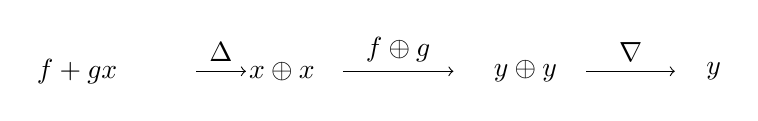
\begin{tikzpicture}[x=1.0em,y=1.0em]
  \node (a) at (0,0) {$f+g\coloneqq x$};
  \node (b) at (7.4,0) {$x\oplus x$};
  \node (c) at (16.2,0) {$y\oplus y$};
  \node (d) at (23.0,0) {$y$};
  \draw[->] (4.3,0) -- node[above]{$\Delta$} (6.1,0);
  \draw[->] (9.6,0) -- node[above]{$f\oplus g$} (13.6,0);
  \draw[->] (18.4,0) -- node[above]{$\nabla$} (21.6,0);
\end{tikzpicture}
\end{rveq}
由引理 2.3.3，\trStable{}\trInfinityCategory{}中的零元素与有限直和下降到其%
\trHomotopyCategory{}上，定义零元素与有限直和。
事实上，\trStable{}\trInfinityCategory{} $A$ 的\trHomotopyCategory{} $\mathrm{h}A$
是\textbf{加性的}（additive），意即
由\cref{eq:sum-of-morphisms} 定义的诸交换幺半群
$\mathrm{h}A(x,y)$ 事实上是阿贝尔群（即每个态射都容许一个加法逆元）
\cite[1.1.2.9]{bib80}。
事实上，Lurie 在 \cite[1.1.2.14]{bib80} 中证明了：若 $A$
是一个\trStable{}\trInfinityCategory{}，则其\trHomotopyCategory{} $\mathrm{h}A$
是 Verdier 意义下的三角范畴 \cite{bib127}。
一个\textbf{三角范畴}（triangulated category）是一个加性范畴 $\mathrm{h}A$，
它容许一个自等价
$\Sigma\colon\mathrm{h}A\rightsquigarrow\mathrm{h}A$，连同指定的\textbf{特异三角形}
（distinguished triangles）
\begin{center}
\begin{tikzpicture}[x=1.3em,y=1.3em]
  \node (x) at (0,0) {$x$};
  \node (y) at (4.4,0) {$y$};
  \node (z) at (8.8,0) {$z$};
  \node (sx) at (13.8,0) {$\Sigma x$};
  \draw[->] (0.6,0) -- node[above]{$f$} (3.7,0);
  \draw[->] (5.1,0) -- node[above]{$g$} (8.1,0);
  \draw[->] (9.5,0) -- node[above]{$h$} (13.0,0);
\end{tikzpicture}
\end{center}
满足六条公理。从 1-\trCategory{}的观点看，特异三角形是附加数据。特别是，
对于一个取值于三角范畴的图表\trCategory{}，不存在定义其特异三角形的典范
方法。Lurie 的洞见在于：\trHomotopyCategory{}所承载的这一结构可以被%
∞-\trCategory{}的一个性质——即稳定性——所捕捉。他宣称 $\mathrm{h}A$ 中的一个
态射三元组 $(f,g,h)$ 是一个\textbf{特异三角形}，如果 $A$ 中存在表示它们的
箭头 $(f,g,h)$，它们装配成如下形式的\trPushout{}矩形：
\begin{center}
\begin{tikzpicture}[x=1.3em,y=1.3em]
  \node (x) at (0,2.2) {$x$};
  \node (y) at (4.6,2.2) {$y$};
  \node (st) at (9.2,2.2) {$*$};
  \node (st2) at (0,0) {$*$};
  \node (z) at (4.6,0) {$z$};
  \node (sx) at (9.8,0) {$\Sigma x$};
  \draw[->] (0.6,2.2) -- node[above]{$f$} (3.9,2.2);
  \draw[->] (5.3,2.2) -- (8.5,2.2);
  \draw[->] (0,1.65) -- (0,0.55);
  \draw[->] (4.6,1.65) -- (4.6,0.55);
  \node at (5.25,1.1) {$g$};
  \draw[->] (9.4,1.7) -- (9.75,0.55);
  \draw[->] (0.55,0) -- (3.9,0);
  \draw[->] (5.3,0) -- node[below]{$h$} (9.1,0);
  \node at (3.9,1.2) {$\scriptstyle\ulcorner$};
  \node at (8.55,1.2) {$\scriptstyle\ulcorner$};
\end{tikzpicture}
\end{center}
于是，在∞-\trCategory{} $A$ 的层面上，把一个箭头 $f\colon x\to y$ 扩充成
特异三角形的方式在本质上是唯一的。特别是，著名的「八面体公理」是命题 4.3.11
的\trPushout{}矩形复合与消去性质的一个推论：给定\trStable{}\trInfinityCategory{} $A$
中一个可复合的态射对 $k\colon w\to x$ 与 $f\colon x\to y$，\trPushout{}方块
之图
\begin{center}
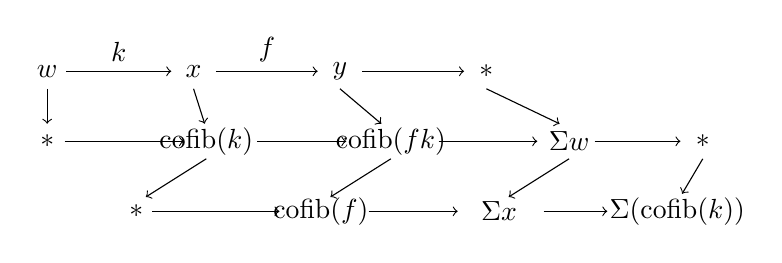
\begin{tikzpicture}[x=1.15em,y=1.15em]
  \node (w) at (0,4.4) {$w$};
  \node (x) at (4.6,4.4) {$x$};
  \node (y) at (9.2,4.4) {$y$};
  \node (st) at (13.8,4.4) {$*$};
  \node (st2) at (0,2.2) {$*$};
  \node (ck) at (5.0,2.2) {$\mathrm{cofib}(k)$};
  \node (cfk) at (10.8,2.2) {$\mathrm{cofib}(fk)$};
  \node (sw) at (16.4,2.2) {$\Sigma w$};
  \node (st3) at (20.6,2.2) {$*$};
  \node (st4) at (2.8,0) {$*$};
  \node (cf) at (8.6,0) {$\mathrm{cofib}(f)$};
  \node (sx) at (14.2,0) {$\Sigma x$};
  \node (sck) at (19.8,0) {$\Sigma(\mathrm{cofib}(k))$};
  \draw[->] (0.6,4.4) -- node[above]{$k$} (3.9,4.4);
  \draw[->] (5.3,4.4) -- node[above]{$f$} (8.5,4.4);
  \draw[->] (9.9,4.4) -- (13.1,4.4);
  \draw[->] (0.55,2.2) -- (4.3,2.2);
  \draw[->] (6.6,2.2) -- (9.4,2.2);
  \draw[->] (12.3,2.2) -- (15.4,2.2);
  \draw[->] (17.2,2.2) -- (19.9,2.2);
  \draw[->] (3.3,0) -- (7.3,0);
  \draw[->] (10.1,0) -- (12.9,0);
  \draw[->] (15.6,0) -- (17.6,0);
  \draw[->] (0,3.85) -- (0,2.75);
  \draw[->] (4.6,3.85) -- (4.95,2.75);
  \draw[->] (9.2,3.85) -- (10.5,2.75);
  \draw[->] (13.8,3.85) -- (16.1,2.75);
  \draw[->] (5.0,1.65) -- (3.1,0.45);
  \draw[->] (10.8,1.65) -- (8.9,0.45);
  \draw[->] (16.4,1.65) -- (14.5,0.45);
  \draw[->] (20.6,1.65) -- (19.95,0.55);
  \node at (2.6,3.3) {$\scriptstyle\ulcorner$};
  \node at (7.6,3.3) {$\scriptstyle\ulcorner$};
  \node at (12.2,3.3) {$\scriptstyle\ulcorner$};
  \node at (4.0,1.1) {$\scriptstyle\ulcorner$};
  \node at (9.6,1.1) {$\scriptstyle\ulcorner$};
  \node at (15.2,1.1) {$\scriptstyle\ulcorner$};
\end{tikzpicture}
\end{center}
定义一个特异三角形
\begin{center}
\begin{tikzpicture}[x=1.3em,y=1.3em]
  \node (a) at (0,0) {$\mathrm{cofib}(k)$};
  \node (b) at (6.6,0) {$\mathrm{cofib}(fk)$};
  \node (c) at (13.2,0) {$\mathrm{cofib}(f)$};
  \node (d) at (21.2,0) {$\Sigma(\mathrm{cofib}(k))$};
  \draw[->] (2.9,0) -- (4.4,0);
  \draw[->] (9.5,0) -- (11.0,0);
  \draw[->] (16.1,0) -- (18.2,0);
\end{tikzpicture}
\end{center}
它与扩充 $k$、$f$ 与 $fk$ 的给定特异三角形相容。
\end{digression}

\subsection*{练习}

\begin{exercise}\label{ex:pointed-initial-terminal-arrow}
在\trHomotopyCategory{}中论证：若一个∞-\trCategory{} $A$ 容许一个\trInitial{}%
元素 $i$ 与一个\trTerminal{}元素 $t$，且存在箭头 $t\to i$，则 $A$ 是一个%
\trPointed{}\trInfinityCategory{}。
\end{exercise}

\begin{exercise}\label{ex:zero-map}
设 $A$ 是一个\trPointed{}\trInfinityCategory{}，$f,g\colon X\to A$ 是%
\trFunctor{}；定义一个典范零映射
\begin{center}
\begin{tikzpicture}[x=1.4em,y=1.4em]
  \node (X) at (0,0) {$X$};
  \node (A) at (3.8,0) {$A$};
  \draw[->] (0.55,0.3) to[bend left=20] node[above]{$f$} (3.25,0.3);
  \node at (1.9,0) {$\scriptstyle\Downarrow\psi_{0}$};
  \draw[->] (0.55,-0.3) to[bend left=20] node[below]{$g$} (3.25,-0.3);
\end{tikzpicture}
\end{center}
使它经过零元素处的\trConstantFunctor{}分解。
\end{exercise}

\begin{exercise}\label{ex:finite-direct-sums}
证明：任何容许二元直和的\trPointed{}\trInfinityCategory{}容许有限直和。
\end{exercise}

\begin{exercise}\label{ex:exact-functors}
\trStable{}\trInfinityCategory{}之间的一个\trFunctor{} $f\colon A\to B$ 是%
\textbf{正合的}（exact），如果它保持零元素以及纤维序列与余纤维序列。
证明：正合\trFunctor{}也保持\trExactSquare{}。
\end{exercise}






